\documentclass[11pt,twoside]{eitExjobb}
\title{Implementing a tool for better obfuscation using overlapping instructions}
%%\documentclass[11pt,twoside,final]{eitExjobb}
% Use final for the final version that will be printed
%%%%%%%%%%%%%%%%%%%%%%%%%%%%%%%%%%%%%%%%%%%%%%%%%%%%
%%\usepackage[Text,Num]{LUfonts}%% LU fonts (local file)
%%%%%%%%%%%%%%%%%%%%%%%%%%%%%
% Nicer fonts
%%\usepackage{pxfonts}
%%\usepackage{mathpazo}
%%%%%%%%%%%%%%%%%%%%%%%%%%%%%
% ���

\usepackage[T1]{fontenc}
\usepackage[normalem]{ulem}
%% Packages used in the thesis
\usepackage{color}
\usepackage{graphpap}
\usepackage{cite}
\usepackage{url}
\usepackage{todonotes}
\usepackage{graphicx}
\usepackage{fancyvrb}

\bibliographystyle{alpha}
\unitlength=1mm
%%%%%%%%%%%%%%%%%%%%%%%%%%%%%%
%%%%%%%%%%%%%%%%%%%%%%%%%%%%%%
%%%%%%%%%%%%%%%%%%%%%%%%%%%%%%
\begin{document}
%%% Title page
\Title{Implementing a tool for better obfuscation using overlapping instructions}
\Author{Erik Nylander\\\texttt{ada09eny@student.lu.se}}
\Date{\today}
\Advisor{Christopher J\"amthagen}
%%\Company{Company\\Address}
\MakeTitlePage
%%%%% Page numbering for front pages
\frontmatter
%%%%% Abstract
\chapter*{Abstract}
This report describes the implementation of a code obfuscation tool using instruction overlapping. Instruction overlapping is a technique used to hide code inside other code to throw off various disassemblers. If a commercial product would be obfuscated using instruction overlapping it could potentially be protected from being copied and spread on the Internet.

The tool was implemented and tested using different programs with varying results. While some tests showed promising results, the tool proved to be lacking in others. To make the tool stronger, improvements has been thought out and suggested.

While there are problems when using instruction overlapping, the technique shows promise and a tool could certainly be implemented. With the suggested improvements, the tool should be able to achieve a satisfying level of obfuscation for any program. 

%% ToC
\tableofcontents
%\cleardoublepage
\listoffigures
\listoftables
\cleardoublepage
%%%%% Page numbering for the main thesis
\mainmatter
%%%%%

\chapter{Introduction}
The software business is a very competitive field because it is very lucrative in this day and age. In order to generate the highest revenue, a software company must provide software that goes beyond what products from other companies are doing. To do so, the source code must be exclusive and only known by people inside the company. The alternative is to have source code that is public domain but provide a service to use the code with that no other company can provide. 

Today it is not sufficient to only worry about other companies stealing or copying code, hackers and piracy is a big problem. It is also not sufficient to keep the source code secret only during the development. When a program is ready for release it is built and packaged and the source code is never made public in clear text. However, when a program is released, the built source code is contained in the executable binaries. These binaries are vulnerable because an adversary can use different kinds of disassemblers to go from the binary hexadecimal codes to assembly code. When the assembly code is made visible to the adversary, it can be analyzed and exploited. 

After the release of a program, usually it takes a couple of weeks or sometimes days for a hacker to copy the program and release it on the Internet. It is not unusual for a program to solely rely on license keys in order to make the program usable only to those who has bought it. The way a hacker can exploit this is to disassemble the binary files, find out how the license key's validity is calculated, write a license key generator that produces a seemingly legitimate serial key by reverse-engineering the validity check. The program can then be released to the public together with the license key generator so that anyone can use the program without buying it, causing a loss in revenue for the developer.

One way of avoiding this problem is to use anti-disassembly. Anti-disassembly is the art of making a program difficult to disassemble and analyse. By utilizing different techniques, a program can be modified so that a disassembler produces erroneus output or no output at all. Several anti-disassembly techniques have been developed and used over the years but the search for better techniques goes on. 

This thesis aims to investigate the use and possibilities of one such technique called \emph{Instruction overlapping}. \emph{Instruction overlapping} exploits the variable length of instructions in the x86 architecture and attempts to hide code inside other code to make a disassembler produce faulty output  while still maintaining the correct behaviour when the program is run. To investigate the practical uses of this technique, a tool will be implemented and tested to determine if \emph{Instruction overlapping} is a viable option for anti-disassembly and also how such a tool could be implemented.


\chapter{Background}
\section{CISC}
CISC (Complex Instruction Set Computer) denotes a series of microprocessor architectures mainly used in personal computers today. When the first CISC processors were launched, memory was expensive so in order to conserve memory space, instructions were designed to take up as little space as possible when used in programs. At the same time, engineers struggled to bridge the semantic gap, meaning the gap between high-level code and assembler code which would allow for better compilers as the assembler code approached high-level functionality. This resulted in a large set of instructions, many of them able to carry out several low level operations such as loading of data from memory, arithmetic instructions and storing of data to memory. In the end, this approach proved to be lacking because it made compilers difficult to implement since there were so many instructions to choose from. Another big problem was that the processors were hard to implement in hardware because the instructions became so complicated. The most important aspects of CISC architectures are as follows:\cite{datorteknik}

\begin{itemize}
\item{An extensive set of instructions to provide a lot of possibilities when coding.}
\item{Powerful instructions performing several low level operations meant to bridge the gap between assembler code and high-level code.}
\item{Instructions of variable length.}
\end{itemize}

\section{RISC}
As the limitations of CISC became more apparent in the 1980s, researchers at University of California at Berkeley and Stanford University started looking for less troublesome, more simple and overall more flexible alternatives. This research resulted in a new type of computer architecture called RISC (Reduced Instruction Set Computer). RISC aimed to make microprocessors easy to implement in hardware and easier to code for by using a much smaller but more straight forward instruction set. The developers of RISC always had the words ``make the common case fast'' in mind while developing. This largely contrasts the way of thinking while developing the older CISC-architecture where the developers aimed to make very powerful and specific instructions in order to make the assembler code more similar to high-level code while using as little memory as possible. The most important aspects of the RISC architecture are the following:

\begin{itemize}
\item{All instructions are of the same length. This makes the instructions easier to decode and it also makes the architecture much simpler to implement in hardware.}
\item{To provide many registers without any special purposes, allowing for variables and temporary calculations to be stored in registers as opposed to being stored in memory resulting in much faster calculations.}
\item{Only certain load and store instructions may access memory. The purpose of this is to reduce the amount of low level operations an instruction can perform which makes more effective use of the ALU while at the same time reducing the complexity of the instructions.}
\end{itemize}

\noindent Even though the RISC architecture had many advantages over CISC, it took a long time for RISC to take its place, mainly because of the lack of software support and the fact that memory was still expensive. Today however, RISC is the most commonly used microprocessor-architecture used overall while CISC still dominates the personal computer-market. Some well known manufacturers of RISC-chips are MIPS, Sun Microsystems(SPARC) and ARM.\cite{datorteknik}

\section{IA-32 architecture}
IA-32 is the third generation of  x86 microprocessor architectures made by Intel. When it was launched in 1985 together with the Intel 80386 microprocessor it was the first 32-bit architecture from Intel, fully backwards compatible with programs made for previous generations of 16- and 8-bit processors. x86 in itself is a CISC architecture which together with the backwards compatibility of IA-32 to its predecessors made for a very complicated platform with an extensive set of instructions with different levels of complexity. Another consequence of this is that the instructions can vary in length from one byte up to fifteen bytes which unintentionally open some interesting possibilities for code obfuscation.. 

With the new 32-bit architecture and Protected Mode, the Intel 80386 could address up to 4 gigabytes of memory. However, when using Protected Mode, all programs are assigned a certain amount of memory to use in order to prevent programs from interfering with each other and any attempt to access memory outside of the allotted amount results in a segmentation fault.

\subsection{The IA-32 instruction set}
Being a CISC architecture, the instruction set for IA-32 contains a very large amount of instructions which can be roughly divided into the following categories:\cite{x86quickguide}\cite{artofassembly} 

\begin{description}
\item[Data movement instructions] Instructions to move data around between memory or registers. 
\item[Arithmetic instructions] These instructions perform arithmetic operations like addition and subtraction.
\item[Logical instructions] Logical instruction perform logical operations such as AND, OR and other bit-operations.
\item[Control flow instructions] These instructions change the control flow of the program.
\item[I/O instructions] I/O instructions gives access to the I/O ports on the processor in order to read data from or write data to peripheral devices.
\item[String instructions] String instructions are used to operate on data in the form of strings of bytes.
\item[Interrupts] Interrupt instructions invoke different kinds of software interrupts in the processor.
\end{description}

\subsection{Looking at an x86 instruction}
The IA-32 instruction format is shown in Table \ref{table:ia32instructionformat}: \\

\begin{table}[h]
\begin{tabular}{|l|l|l|l|l|l|}
\hline
Prefix & Opcode & Mod-Reg-R/M & SIB & Displacement & Immediate \\ \hline
1-4 bytes & 1-2 bytes & 1 byte & 1 byte & 1-4 bytes & 1-4 bytes \\
\hline
\end{tabular}
\caption{The IA-32 instruction format}
\label{table:ia32instructionformat}
\end{table}

\begin{description}
\item[Prefix] This is an optional field used to add prefixes to certain instructions in order to override segment sizes, operand sizes and so on.
\item[Opcode] The opcode consists of 1-2 bytes and is the instruction code that determines the type of instruction. Some instructions only contain this field.
\item[Mod-Reg-R/M] The Mod-Reg-R/M byte is used in a couple of different ways, mainly to determine if an instruction will access memory or registers. This field will be explained in more detail later.  
\item[SIB] SIB stands for \emph{Scale-Index-Base} and is used to enable index-based addressing of memory. This field will be explained in more detail later.
\item[Displacement] The displacement field is used to access memory with a displacement. If the Mod-Reg-R/M-byte gives the register that the memory address will be collected from, the displacement field will determine a value to add to the address before accessing the memory.
\item[Immediate] Instructions that uses some kind of immediate value gathers this value from this field instead of picking one from a register or memory.
\end{description}

\subsubsection{The Mod-Reg-R/M byte}
The Mod-Reg-R/M byte consist of three groups of bits that together determines what kind of data that the instruction is accessing, see Table \ref{table:modregrmbyte}. These groups are explained below:\\

\begin{table}[h]
\begin{tabular}{|l|l|l|}
\hline
Mod & Reg & R/M \\
\hline
2 bits & 3 bits & 3 bits \\
\hline
\end{tabular}
\caption{Format of the Mod-Reg-R/M byte}
\label{table:modregrmbyte}
\end{table}


\noindent \uline{Mod}\\
The two \emph{Mod} bits determines if the instruction shall access memory at an address stored in a register and also if a displacement shall be added to the address.\\
\begin{description}
\item[00] The processor will use indirect addressing mode. The address will be collected from the register specified by the \emph{R/M} bits. Two exceptions are when the \emph{R/M} field is \emph{100} or \emph{101}.  
\item[01] Indirect addressing mode but an 8-bit displacement will be added to the address before it is dereferenced.
\item[10] Indirect addressing mode but a 32-bit diplacement will be added to the address before it is dereferenced.
\item[11] Direct addressing mode, no memory will be acccessed. Both the \emph{Reg} and \emph{R/M} fields will denote registers.
\end{description}

\noindent \uline{Reg}\\
The \emph{Reg} field will denote a register: \\ 000 - eax, 001 - ecx, 010 - edx, 011 - ebx, 100 - esp, 101 - ebp, 110 - esi, 111 - edi.\\


\noindent \uline{R/M}\\
The \emph{R/M} field will denote a register just like the reg field. It also denotes the register from which an address will be dereferenced. There are two exceptions to this, namely if the mod bits are 00 and if the \emph{R/M} bits are \emph{100}, then the SIB byte will be used when accessing memory or when the \emph{R/M} bits are \emph{101}, then a displacement value will be dereferenced instead.

\subsubsection{The SIB byte}
The SIB byte like the Mod-Reg-R/M byte also contains three fields of bits called \emph{Scale}, \emph{Index} and \emph{Base}, see Table \ref{table:sibbyte}. As mentioned before, this byte enables index-based memory access. When the SIB byte is used, the address being accessed will be calculated as follows:
$Base + Scale*Index$. The fields in the SIB byte will be explained below:\\

\begin{table}[h]
\begin{tabular}{|l|l|l|}
\hline
Scale & Index & Base \\
\hline
2 bits & 3 bits & 3 bits \\
\hline
\end{tabular}
\caption{Format of the SIB byte}
\label{table:sibbyte}
\end{table}


\noindent \uline{Scale}\\
The two \emph{Scale} bits determines what value the \emph{Index} value will be multiplied with.\\
\begin{description}
\item[00] \emph{Index} will be multiplied by 1.  
\item[01] \emph{Index} will be multiplied by 2.
\item[10] \emph{Index} will be multiplied by 4.
\item[11] \emph{Index} will be multiplied by 8.
\end{description}

\noindent \uline{Index and Base}\\
The \emph{Index} and \emph{Base} fields both denotes registers encoded in the same way as the \emph{Reg} and \emph{R/M} fields in the Mod-Reg-R/M byte. \cite{bittwiddling}\cite{assemblylanguagex86}



\section{Disassemblers}
There are generally two different kinds of disassemblers namely static disassemblers and dynamic disassemblers. Static disassemblers use either a linear sweep algorithm or a recursive traversal algorithm to decode the instructions in a program. A linear sweep disassembler works in such a way that it reads the program byte after byte, decoding instructions as they come along. A clear advantage with this approach is that the entire program can be disassembled in a single sweep. It is also fairly quick since it only depends on the size of the program. The perhaps most critical disadvantage this approach has is that it does not take the control flow of the program in to account causing it to misinterpret things like data embedded in the stream of instructions.

Recursive traversal disassemblers works such that whenever they encounter a function call or a branch instruction it calculates the possible target address of the instruction, marks the current address as visited and then proceeds to recursively call its disassembler function with the potential target addresses of the current instruction. If it encounters an address that has already been visited, the function returns. This enables the disassembler to avoid interpreting embedded data as executable instructions.

A dynamic disassembler executes the code at the same time as it disassembles the instructions by using an attached debugger, allowing it to follow the control flow of the program by executing branch instructions and function calls. 

Since an analyst can use different kinds of disassemblers, the obfuscator must take the weaknesses of each in account when obfuscating the code in order to achieve a high level of obfuscation to confuse the analyst.

\chapter{Code obfuscation}
\section{What is code obfuscation}
Obfuscating code is the action of deliberately making code harder to analyze, interpret and recreate. In the case of machine code, the idea is to make the code hard to disassemble correctly and hard for humans to read and understand once it has been disassembled. The creator of some program can choose to obfuscate their code for a variety of reasons, both benign and malevolent e.g., a legitimate programmer may want to hide certain parts of a program, for example which ports the program listens to or the algorithm that determines if a serial code is correct while on the other hand  a hacker might  want to make his virus harder to analyze which could delay the analysis of the virus and the creation of a fix which in turn would let the virus infect a larger number of hosts. By achieving a high level of obfuscation, the risk of a program getting cracked, copied and spread on the internet is greatly reduced. It will also be less susceptible to hacker attacks since an adversary will have a difficult time finding security flaws to exploit.

\section{Some obfuscation techniques}
Over the years, several obfuscation techniques have been invented and employed, ranging from simple tricks to confuse linear sweep disassemblers to sophisticated self modifying code. Some notable approaches will be presented below.

\subsection{Junk byte insertion}
This obfuscation technique aims to exploit the weakness of linear sweep disassemblers by embedding data among the executable instructions. Upon disassembly, the disassembler will interpret the junkbyte as the opcode to the start of an instruction, which could cause the following bytes to be interpreted as the rest of the instruction. This would make the program look completely different from the program written without the junkbyte. Note that a recursive traversal disassembler follow the control flow of the program so that it never encounters the junk byte. An example of junk byte insertion is displayed below.\cite{instructionoverlapping}
\\
\\
Consider the following code:
\begin{verbatim}
jmp label               eb 01
db 0x8d                 8d    # junk byte

label:
xor eax, 0x12345678     35 78 56 34 12
int 0x80                cd 80
\end{verbatim}
\noindent After assembling the code above and then using the GNU Assembler \texttt{objdump}\cite{objdump} on it we see that the linear sweep algorithm produces the following code:

\begin{verbatim}
$ objdump -D -b binary -mi386 -M intel example.o
   0:	eb 01                	jmp    0x3
   2:	8d 35 78 56 34 12    	lea    esi,ds:0x12345678
   8:	cd 80                	int    0x80
\end{verbatim}

\noindent Here it is very clear that the linear sweep algorithm in \texttt{objdump} interpreted the data byte 0x8d as the the opcode for the x86 \emph{Load Effective Address} instruction making the disassembled code look different from the code that was actually written. An important thing to note is that the junk byte must be placed so that it will never be reached, potentially causing the program to crash. Another important thing to notice in this example is the fact that the instruction \texttt{int 0x80} appears in both code snippets. This is due to the fact that the disassembler tends to synchronize with the correct code in a few instructions (one in this case) because of the variable length of x86 instructions.  

\subsection{Opaque predicates}
Opaque predicates is a technique used to fool recursive traversal disassemblers and can be used together with junk byte insertion. The idea is to convert unconditional jump instructions into conditional jump instructions but make it so that the jump is always taken at runtime. This forces the recursive traversal algorithm to consider both the target as well as the next instruction after the jump. By placing junk bytes directly after the jump instruction, the disassembler can be tricked into producing erroneous code.\cite{instructionoverlapping}

Modifying this technique could also fool a dynamic disassembler. Since a dynamic disassembler will disassemble the code while it is being run, it will only encounter the legitimate code and never reach the junk byte. However, this could be overcome by making the seemingly unconditional jump conditional. This might seem confusing but if one were to make the conditional jump depend on the fact that a debugger was present or not, one could make the jump be not taken if that was the case. Then the dynamic disassembler would be forced to disassemble the junk byte, making it produce faulty code.


\subsection{Instruction embedding}
Instruction embedding\cite{instructionembedding} is an interesting obfuscation technique because it effectively hides one or more instructions inside another instruction. An instruction \emph{a} embeds an instruction \emph{b} if the last \emph{x} bytes of \emph{a} consist of all the bytes in \emph{b}. The most important part of any obfuscation technique is to not change the behaviour of the program, luckily, the x86 architecture allows jumps into the middle of an instruction. This means that a jump can be made into the embedding instruction so that the next instruction to be run is actually the embedded instruction.

Since the embedding instruction must be able to contain the entirety of the embedded instruction there are constraints on what instruction can be embedded and which instructions they can be embedded in. The best instructions to use as embedding instructions are those that utilize both a 32-bit displacement value and a 32-bit immediate value, then it will contain 8 bytes that are fully customizable which means that an instruction with the length of 8 bytes can be embedded. Consider the following instruction:

\begin{verbatim}
    lea esi, 0x12345678                     ; 8d 35 78 56 34 12
\end{verbatim}

\noindent If the byte \texttt{8d} would be removed, the following instruction would be found:

\begin{verbatim}
    xor eax, 0x12345678                     ; 35 78 56 34 12
\end{verbatim}

\noindent In this example, the instruction \texttt{xor eax, 0x12345678} is embedded in the instruction \texttt{lea esi, 0x12345678}.

\subsection{Using cryptographic hash functions or pseudo-random number generators}
These two approaches both stem from the same idea, namely to generate the code at runtime so that it is never visible to an analyst using a static disassembler. Because the code is generated first when the program is run, it is only present at runtime and only in memory, which means that there is no code to analyze when the program is not being run.

In the case of using pseudo-random number generators, the basic idea is to find a seed \emph{s} to a built-in pseudo random number generator \emph{G} on the host such that a number of consecutive calls to \emph{G} will generate the desired bytes. This is often very hard to do since the probability of finding such a seed is very small, especially as the number of desired bytes grow in size. Because of this the method can be altered by using different kinds of mappings between the generated numbers and the desired bytes.\cite{prng}

When using cryptographic hash functions, the idea is similar. By using some key combined with a salt value together with some cryptographic hash function, a sequence of bytes will be generated. The goal is to find the key, a salt and a hash function such that they together generate the bytes that make up a program. Like the case when using pseudo-random number generators this is very hard to achieve which is why this form of anti-disassembly is rarely used.\cite{chf}

Both of these approaches depend on finding certain values to make them work. The only way to do this is by doing an exhaustive search for suitable values which in turn requires a lot of computing power. If this search space could be divided among a large amount of hosts, time it would take to obtain the desired values would be greatly reduced. An interesting thing to note is that this kind of distributed computing mainly exist in botnets and that a programmer with a botnet at his disposal usually has malevolent purposes in mind. 

\section{Instruction overlapping}
Instruction overlapping is the obfuscation technique of which the main focus of this thesis lies on. It is similar to instruction embedding in that it hides instructions inside others but it is also more advanced and a more elegant solution. In the case of instruction embedding, an instruction hides another and a jump is needed to execute the hidden instruction. This requires a large amount of jump instructions when a large amount of instructions are hidden which could seem suspisious to an analyser. At the same time, it would not stand a chance against a dynamic disassembler since the control flow of the program is followed and only the instructions executed are disassembled. Instruction overlapping in its simplest form attempts to overcome the former of this problem by making the code look normal. With a bit of tweaking it can also overcome the second problem by making the disassembler execute the non-hidden code.

The main difference between instruction overlapping and instruction embedding is that instruction embedding hides one instruction inside another while in instruction overlapping, several instructions can be hidden inside several others. The main idea is that when looking at a program as a stream of bytes, if the program were to be run starting with the first byte in the stream, one execution path would be executed while if the program were to be run starting at an offset from the first byte, another execution path would be executed. The perfect scenario for this technique would be to have two completely executable paths (non of the executions paths crasches the program) so that the execution path starting at the first byte is the visible code (to the analyst) and the executions path starting at an offset is the hidden code. If this result was achieved, only one jump instruction into the hidded execution path would be needed to run the program as opposed to the case with instruction embedding where serveral jumps were needed. This would make the program look natural and not as suspisious which solves the problem with strange looking code when using instruction embedding.\cite{instructionoverlapping}

\subsection{Overlapping instructions}
Instructions are overlapping if one sequence of instructions $a$ can be extracted from another sequence of instructions $b$ by removing one or more of the bytes making up sequence $b$. For example, consider the following instructions:

\begin{verbatim}
    test dword [edi+0x10c383ff], 0x5b8      ; f7 87 ff 83 c3 10 b8 05 00 00
    add [ebx-0xf7cfc40], al                 ; 00 83 c0 03 83 f0
    add al, [ecx]                           ; 02 01
    nop                                     ; 66 90
\end{verbatim}

\noindent If the instructions above make up sequence $b$, then sequence $a$ can be found inside $b$ by removing the bytes \texttt{f7 87 ff}:

\begin{verbatim}
    add ebx, 0x10                           ; 83 c3 10
    mov eax, 0x5                            ; b8 05 00 00 00
    add eax, 0x3                            ; 83 c0 03
    xor eax, 0x2                            ; 83 f0 02
    add [esi-0x70], esp                     ; 01 66 90
\end{verbatim}

\subsection{Main Execution Path and Hidden Execution Path} 
As mentioned before, instruction overlapping relies on having two executable paths in one program, the \emph{Main-Executaion-Path}(from here on called MEP) and the \emph{Hidden-Execution-Path}(from here on called HEP). The MEP is the path visible to an analyst and the HEP will consist of the program that is hidden. In the example in the previous section, sequence $b$ is the MEP and sequence $a$ is the HEP.

Upon execution, to access the HEP, a jump instruction has to be placed before the MEP to change the control flow of the program so that program counter will find the next instruction starting at the first byte of the HEP. This will allow the HEP to be executed while remaining hidden if the program is disassembled using a linear sweep disassembler. 

To fool a dynamic disassembler is a little more difficult but it is possible. To do this, the MEP has to be executed since a dynamic disassembler only disassembles the instructions that are run. Analysis of programs are often done on virtual machines to protect the host system from potentially harmful programs. This is very good for the sake of instruction overlapping since there are ways for a program to find out if it is run with a debugger attatched or on a virtual machine. The jump into the HEP can then be made to depend on this fact\cite{redpill}\cite{gdbhaxx}\cite{ollydbghaxx}.

Unfortunately this makes up one of the main challenges when using instruction overlapping namely that the MEP must be able to run without crashing. Since the MEP is generated by inserting bytes in front of the HEP, there is little control to be had over the instructions in the MEP once the bytes to put before the HEP has been chosen.  Certain type of instructions are not suitable in a MEP, memory accessing instructions for example could very easily make the program crash. Other undesireable instructions are jump instructions  and interrupts.

The other main challenge is that because of the variable instruction length in the x86 architecture, the MEP tends to synchronize with the HEP after a number of instructions. This is a problem because once the MEP has synchronized with the HEP, the remaining instructions of the program are out in the open. 

The intended behaviour when using instruction overlapping is described in Figure \ref{fig:instructionoverlappingflowchart}.

\begin{figure}[here]
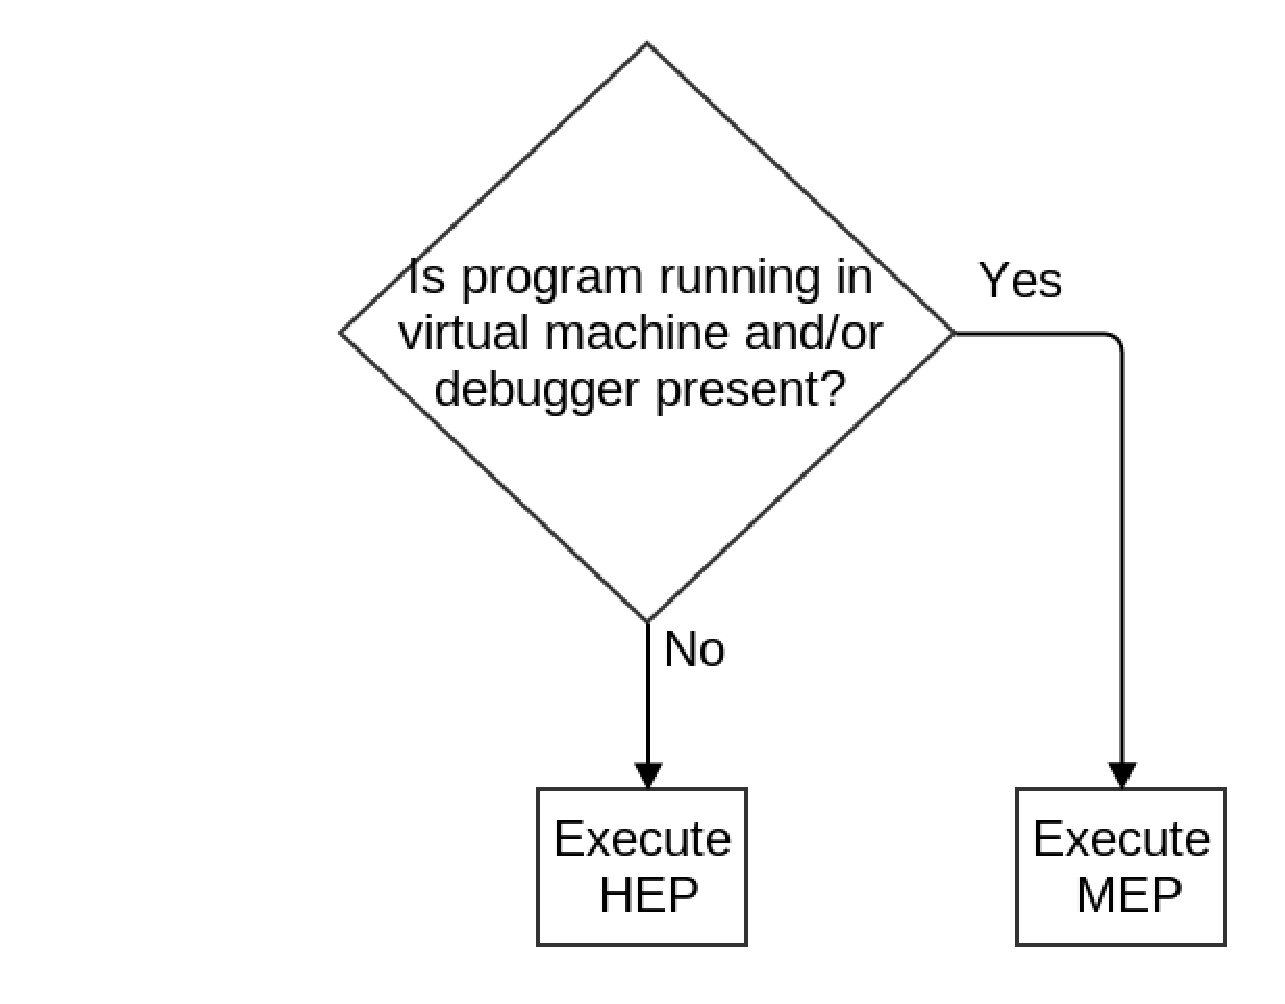
\includegraphics[scale=0.4]{instructionoverlapping.eps}
\caption{Flowchart for the behaviour when using instruction overlapping}
\label{fig:instructionoverlappingflowchart}
\end{figure}


\subsection{Instruction overlapping using NOP instructions} 
One way of achieving instruction overlapping is by using \emph{nop} instructions\cite{instructionoverlapping}. The \emph{nop} instruction is interesting because while it can be encoded as \texttt{0x90} it can also be encoded using up to 15 bytes. Consider the following instruction and its encoding: 
\begin{verbatim}
    nop word ptr [eax+eax + 0x00000000]}; 66 0f 1f 84 00 00 00 00 00         
\end{verbatim}

\noindent Because the \emph{nop} instruction does not alter the state of the processor other than increasing the program counter, it will not access any memory even though it has a memory operand. What this means is that the last five bytes of the instruction can be chosen arbitrarily meaning that the nine byte \emph{nop} can be used for instruction overlapping. The reason for not using the 15 byte encoding is that the additional bytes are static and can not be assigned arbitrary values.

The idea is to hide the HEP instructions inside the \emph{nop} instructions. This ensures that the MEP is runnable but it raises the question of how to make the HEP able to run as well. By just embedding the HEP instructions inside \emph{nop} instructions, all that is achieved is non functioning \emph{instruction embedding}. What is needed is something to glue the HEP together and make it runnable. In \cite{instructionoverlapping} the proposed way of doing this is to use so called \emph{wrapping instructions}. The wrapping instruction will be placed between the instructions in the HEP to serve as a bridge between the \emph{nop} instructions in the MEP. This is best explained by considering the format of the MEP instructions to look like this: \texttt{XX YY ZZ} where \texttt{XX} are the prefix and opcode bytes, \texttt{YY} are the arbitrarily chosen bytes which makes up the HEP instruction and \texttt{ZZ} is preferably the last byte in the MEP instruction so that it together with \texttt{XX} make up the wrapping instruction. Then the MEP will look like this:

\begin{verbatim}
    XX YY ZZ  ; nop containing HEP instruction
    XX YY ZZ  ; nop containing HEP instruction
    XX YY ZZ  ; nop containing HEP instruction
    ...
\end{verbatim} 

\noindent The HEP will then look like this:

\begin{verbatim}
    YY        ; HEP instruction
    ZZ XX     ; Wrapping instruction
    YY        ; HEP instruction
    ZZ XX     ; Wrapping instruction
    YY        ; HEP instruction
    ZZ XX     ; Wrapping instruction
    ...
\end{verbatim}

\noindent Ideally the wrapping instruction is one that does not affect the behaviour of the HEP such as \emph{test} or \emph{cmp}. 

An example of this approach will be presented below. Consider the following code:

\begin{verbatim}
    mov ax, 0x15                       ; 66 b8 15 00
    mov bx, 0x1                        ; 66 bb 01 00
    and eax, ebx                       ; 21 d8
\end{verbatim}

\noindent Using \emph{test} as the wrapping function, the MEP will look like this:

\begin{verbatim}
    nop word ptr [esi - 0x56ffea48]    ; 66 0f 1f 84 66 b8 15 00 a9
    nop word ptr [esi - 0x56fffe45]    ; 66 0f 1f 84 66 bb 01 00 a9
    nop word ptr [ecx - 0x6f6f6f28]    ; 66 0f 1f 84 21 d8 90 90 90
\end{verbatim}

\noindent The HEP will then look like this: 

\begin{verbatim}
    mov ax, 0x15                       ; 66 b8 15 00
    test eax, 0x841f0f66               ; a9 66 1f 0f 84
    mov bx, 0x1                        ; 66 bb 01 00
    test eax, 0x841f0f66               ; a9 66 1f 0f 84
    and eax, ebx                       ; 21 d8
    nop                                ; 90
    nop                                ; 90
    nop                                ; 90
\end{verbatim}

\noindent Note that the last three \emph{nop} instructions were added to stop the overlapping.

While this approach ensures that the MEP does not crash, it is not very powerful since the longest instruction that can be hidden has the length of four bytes unless the last byte is suitable for a wrapping instruction in which case the length is five bytes. Other weaknesses are that the MEP code looks very suspicious containing only \emph{nop} instructions and that the HEP gains unecessary instructions.  

\subsection{A more dynamic solution}
A stronger way to achieve instruction overlapping is to iteratively insert bytes in front of the HEP. With a little luck this could make the code overlap and the MEP would end up looking a lot more natural since it would be made up of actual real instructions instead of just \emph{nop} instructions. The first example on instruction overlapping in this report was achieved using this approach. 

The problems with this way of doing things are those that arise when using instruction overlapping in itself, namely to make the HEP and MEP runnable as well as obfuscating a whole program  without having the MEP synchronize with the HEP.

To use this technique and deal with the problems that arise, a tool could be used. Such a tool would have to be able to iteratively insert bytes in front of the program that is to be ofuscated. It must then look at which inserted bytes makes the MEP synchronize with the HEP in the most instructions. When the best bytes have been chosen, the tool has to be able to deal with potential problems such as instructions that makes the MEP crash and so on. 

In short, the problems that a tool needs to be able to handle are when there are instructions accessing memory in the MEP or instructions that change the control flow of the program in the MEP. It also needs to be able to keep the MEP from synchronizing with the HEP.

In the next chapter the implementation of such a tool will be described.

\chapter{Implementation}
\section{Programming Language}
The tool was implemented using C++ with some additional C-libraries. The choice of programming language largely depended on three main factors; speed, flexibility and convenience. C++ was the natural choice because it offers the convenience of the C++ standard libraries which offer good and well implemented container classes and iterators while still maintaning C-like performance.

\section{Main features}
The main features considered for the tool were:

\begin{itemize}
\item{Being able to parse and represent a program}
\item{Being able to insert one or more bytes before the instructions in the HEP to optain a MEP}
\item{Being able to determine which of the inserted bytes generates the longest and best MEP}
\item{Swapping instructions in the HEP if illegal or unsuitable instructions are found in the correspondig place in the MEP}
\item{Compensating for memory access in the MEP}
\item{Emulate the instructions in the MEP and determine if a jump instruction is legal or not if one is found in the MEP}
\end{itemize}

\noindent All of these features were fully implemented or implemented to an extent in the final product. 

\section{Usage}
The tool was implemented so that a specific input generates an output in the form of a template for the obfuscated program generated from the input.  

\subsection{Input}
The intended input for the tool is a file containing the bytes representing an assembled program. The input file is assumed to be assembled in a way such that only the representation of the instructions are present in the input file, i.e. no code to make the program runable are added when the instructions are assembled.

\subsection{Ouput}
The output of the tools is presented as a template for the obfuscated program that was generated from the input file. It contains aside from the instructions a data section where data is allocated, a preface part and a memory adjustment part. The two latter parts will be explained further on.

\section{The algorithm}
The main steps of the algorithm implemented in the tool currently is described in Figure \ref{fig:mainsteps}. The algorithm is described in more detail in the pseudo code below:

\begin{Verbatim}[fontsize=\tiny]
Read and parse input file. Store in HEP vector
Do preface substituting 32 bit lea instructions

If mov substitution parameter is set:
	Substitute all 32 bit mov instruction in HEP vector

Build vector containing all possible starting bytes between 00 and FFFFFF

while no good MEP is found:
	for each starting bytes:
		Copy HEP bytes to MEP
		Insert starting bytes first in MEP
		Check how many instructions are hidden and save the 
		largest number

		Remove starting bytes in MEP

	for each starting bytes:
		Remove starting bytes with fewer hidden instructions 
		than the maximum

	for each starting bytes:
		Copy HEP bytes to MEP
		Insert starting bytes first in MEP
		Calculate number of memory accesing instructions using
		registers to access memory and save minimum
		Remove starting bytes in MEP

	for each starting bytes:
		Remove starting bytes with more than the minimum amount
		of registers to access memory 

		Remove starting bytes generating MEPs containing 
		instructions using SIB bytes

	if starting bytes is empty:
		insert nop instruction first in the HEP and loop
	else:
		break 

Insert last starting bytes before the HEP

Adjust for memory access

Print template for obfuscated program

\end{Verbatim}

\begin{figure}[here]
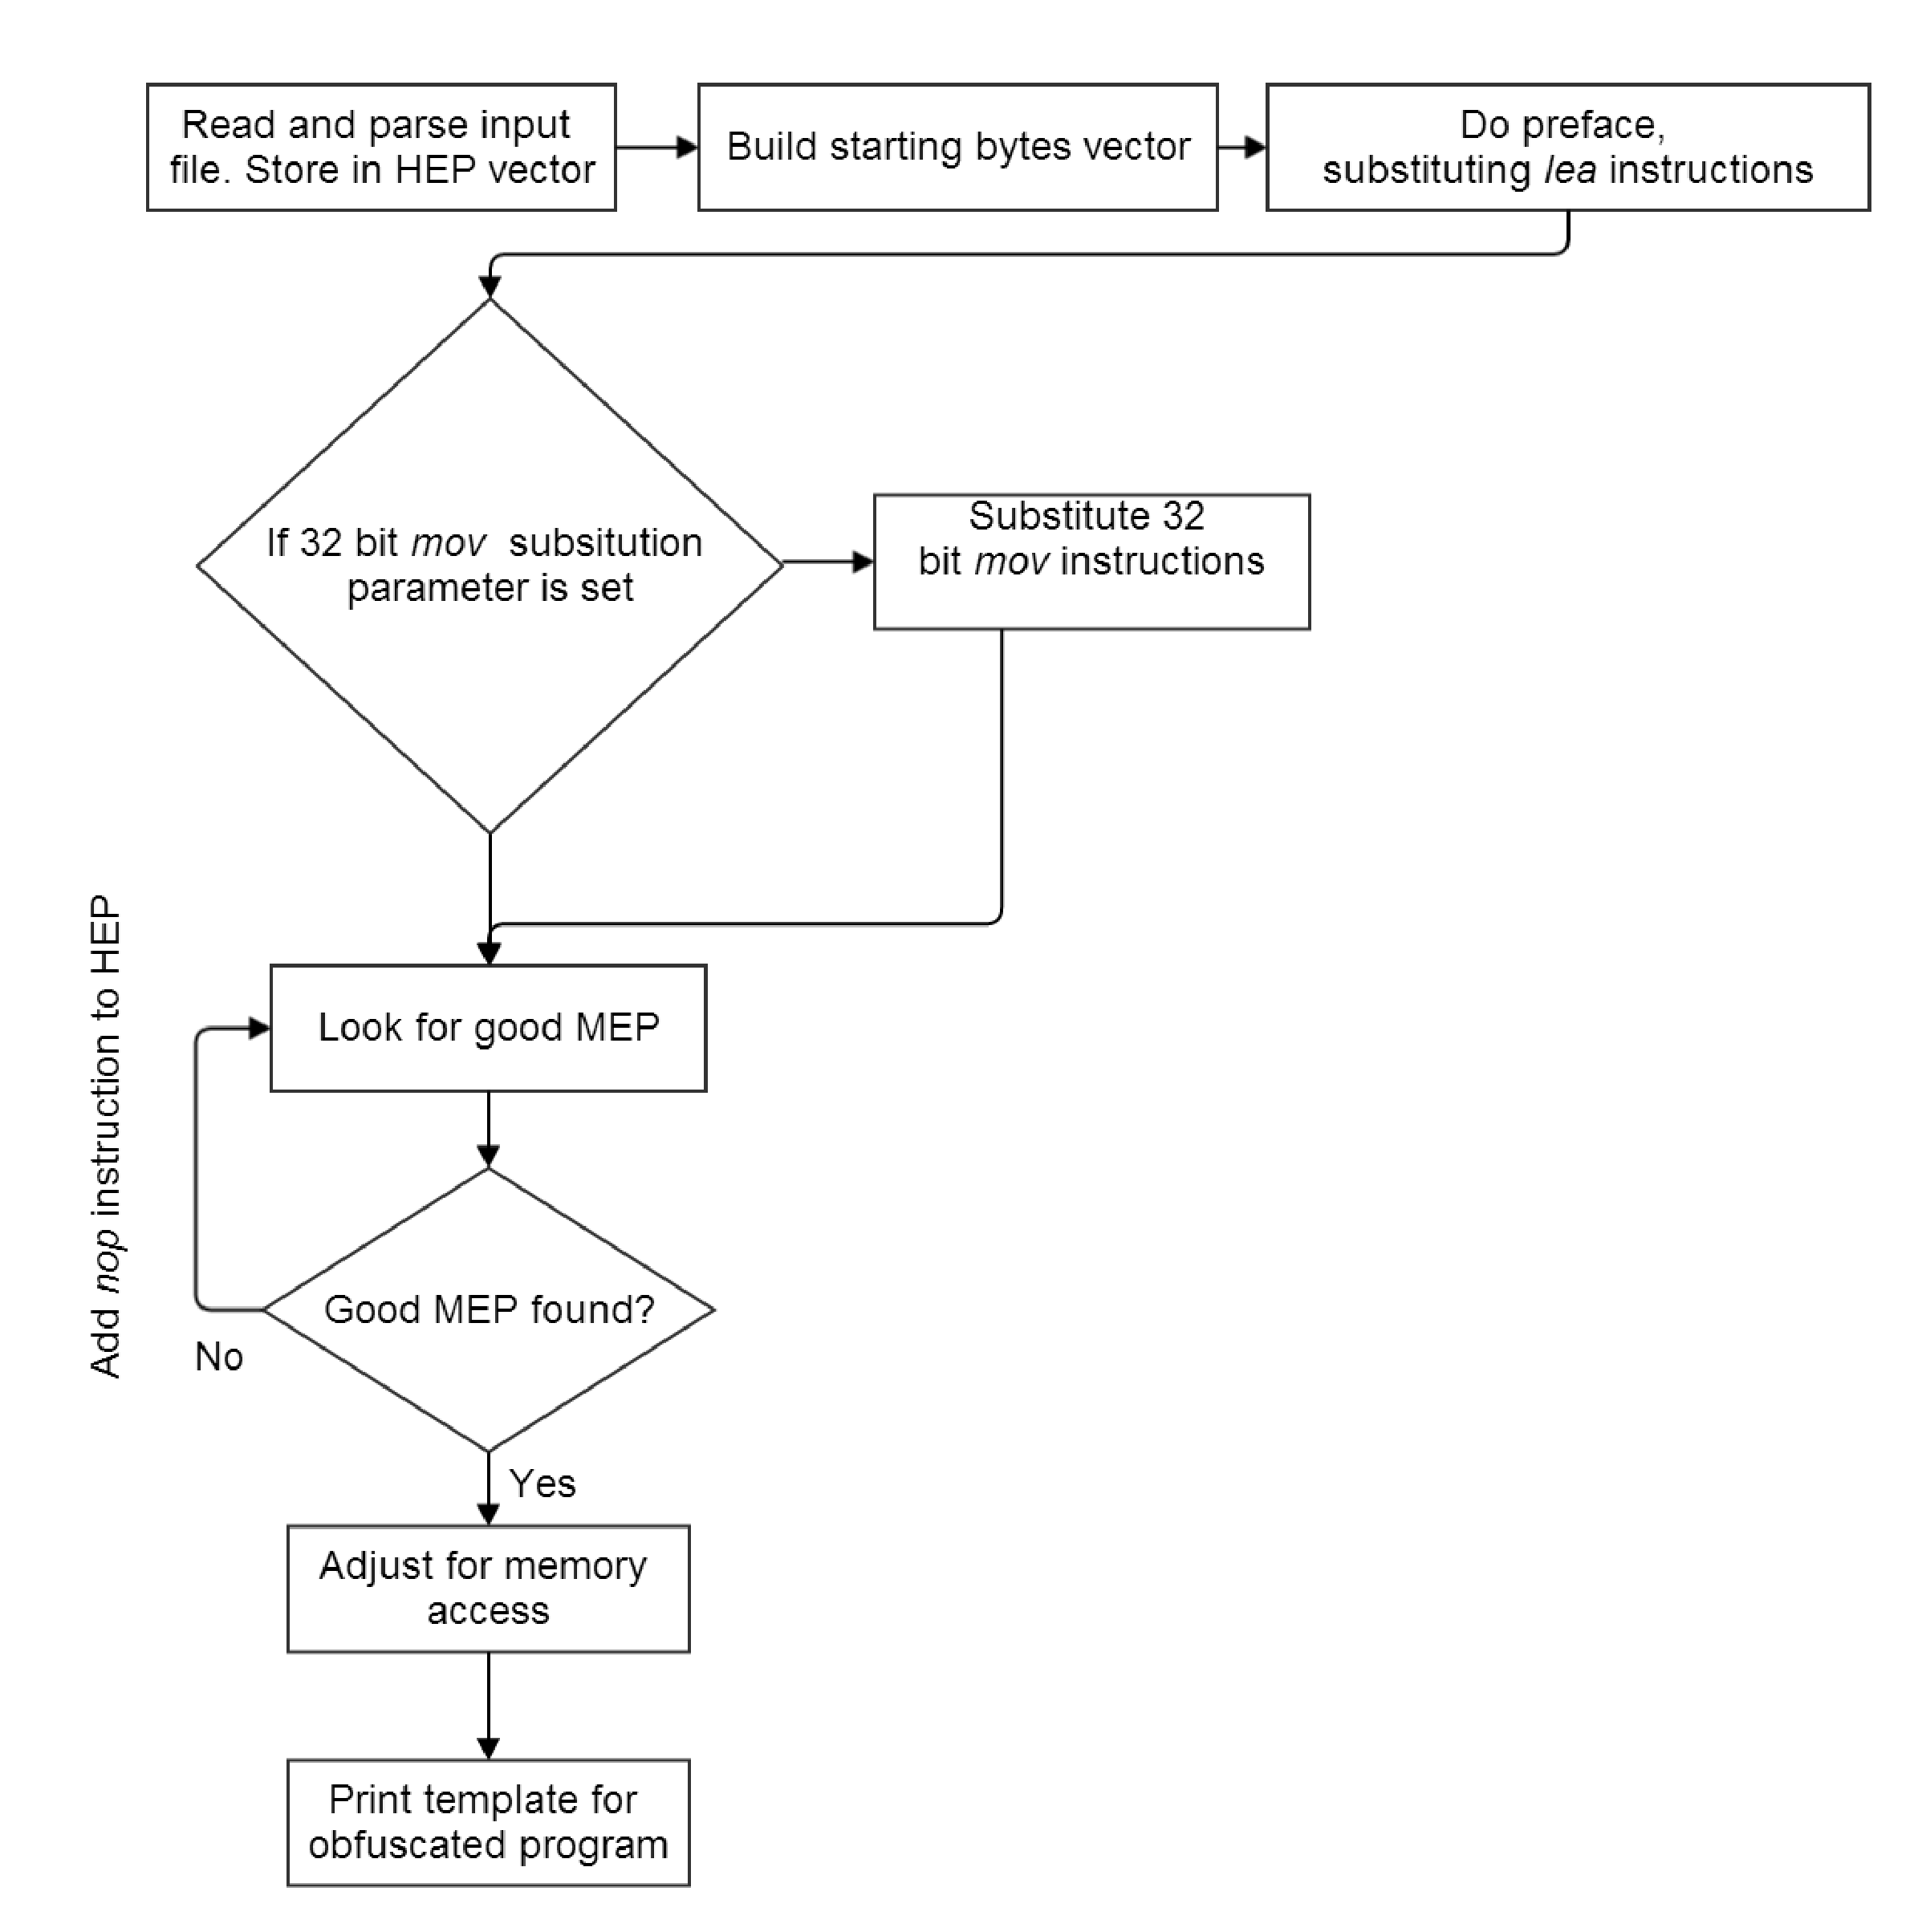
\includegraphics[scale=0.32]{flowchart.eps}
\caption{Flowchart for the main steps of the algorithm}
\label{fig:mainsteps}
\end{figure}

\noindent The algorithm above is the one used in the current implementation. The ideal algorithm for the tool is described below:

\begin{Verbatim}[fontsize=\tiny]
Read and parse input file. Store in HEP vector

Build vector containing all possible starting bytes between 00 and FFFFFF

for each starting bytes:
	Copy HEP bytes to MEP
	Insert starting bytes first in MEP
	Check how many instructions are hidden and save the 
	largest number

	Remove starting bytes in MEP

for each starting bytes:
	Remove starting bytes with fewer hidden instructions 
	than the maximum

for each starting bytes:
	Copy HEP bytes to MEP
	Insert starting bytes first in MEP
	Calculate number of memory accessing instructions and keep track
	of what registers they use.

	remove starting bytes in MEP

Find what starting bytes generating the MEP(s) not using a register
for memory access more than once

if found:
	Pick the best starting bytes and insert first in the MEP
else:
	Pick the second best starting bytes and insert first in the MEP

Optimize_MEP:
while MEP contains problematic instructions and MEP synchronizes with HEP
      and threshold not reached:
	Look for instructions causing problems(Instructions using 
	SIB bytes, instructions causing the MEP to synchronize with 
	the HEP, unconditional jump instructions, etc)
	if found:
		Replace instruction causing the problem in the HEP
	if conditional jump found:
		Emulate instructions before jump instruction and check flags
		if the jump will be taken:
			Replace instruction in HEP causing the jump
		else:
			Proceed

If threshold was reached:
	If MEP still synchronizes with HEP:
		Generate new MEP by inserting new starting bytes before the 
		synchronizing instruction.
		GOTO Optimize_MEP

Adjust for memory access
Print template for obfuscated program adding code for fooling
dynamic disassemblers.
\end{Verbatim}

\section{Parsing and representing a program}
In order to perform operations on a program it needs to be parsed and represented in some way. This part is done in two steps in the tool, first the input file is read and the bytes are stored in a \texttt{vector}, then the bytes are parsed and stored in \texttt{Instruction} objects. 

Since the parsing and representation of x86 instructions would be very time consuming to implement, two different third party C libraries were used, Udis86 and Libemu. 

\subsection{Udis86}
Udis86\cite{udis} is a disassembler library for x86 written in C. It is used to disassemble a stream of bytes and presenting them result both in hexadecimal byte form aswell as in assembly language. It can disassemble bytes coming from either a byte array or directly from a file. In the tool it is used to read a file and return the bytes and to present the output.


\subsection{Libemu}
Libemu\cite{libemu} is a C library used for emulation. It provides the tools to build code analysis programs tailored to specific needs. The library contains an advanced emulator capable of executing a stream of instructions and present the resulting outcome. Alongside the emulator, Libemu offers debugging capabilities.

The tool uses Libemu to parse a stream of bytes and store them in Libemu's internal instruction object. The reason for using an instruction object as opposed to only using the bytes and derive the data necessary from them is that this offers an extra layer of abstraction so that all the instructions can be handled the same way instead of having to utilize ad-hoc style handling for each different type of instruction. The tool wraps the internal instruction object to add some capabilities.

\section{"Preface"}
Some instructions are very long, therefore they are difficult to hide. At the same time they often seem to make the MEP sync with the HEP. In order to avoid this behaviour the tool uses a few tricks to substitute these kinds of instructions by moving them out of the HEP and replace them with other instructions that makes the program behave the same but makes the HEP easier to hide. 

After the input file has been read and parsed, a function called \texttt{doPreface()} is called. This functions loops through the instructions and looks for certain kinds of instructions. If one is encountered, it is substituted for one instruction in the Preface part of the program and one instruction in the HEP. How this is done is different for different kinds of instructions.  

\subsection{Workaround for lea instructions}
The \emph{Load Effective Address} or \emph{lea} instruction loads an address and places it in a register. For example: \texttt{lea eax, [somedata]} computes the address of the source operand \texttt{somedata} and stores it in the destination register, \texttt{eax} without actually accessing the memory. 

If the address of \texttt{somedata} in the example above was \texttt{0x12345678}, the instruction would be encoded as follows: \texttt{8d 05 78 56 34 12}. This instruction is the 6 bytes long which can be hard to hide. 

What happens in \texttt{doPreface()} when it encounters a similar \emph{lea} instruction is that it removes the instructions from the HEP. It then proceeds to add a \emph{lea} instruction with the same destination register but with the label of the data minus 1 as the source operand. After that, an ADD instruction adding 1 to the destination register of the \emph{lea} instruction is added to the HEP where the original \emph{lea} instruction was located. For example:

\begin{verbatim}
    lea eax, [somedata]
\end{verbatim}

\noindent becomes:

\begin{verbatim}
preface:
    lea eax, [somedata-1]

hep:
    add eax, 1
\end{verbatim}

\noindent The result is that the program behaves like it did prior to the change but the HEP will be easier to hide while the \emph{lea} instruction and the data which address is loaded is somewhat hidden.

The use of a label yields a problem that also affects other parts of the tool. Since the input file is derived from a file written in assembly language, the labels are translated into memory addresses when the file is assembled and because the assembler file is assumed to be assembled without any headers to make the program runable, the address that the label is translated into will not be correct when the output from the tool is run. Because of this, all use of labels has to be done manually after the output has been generated before the obfuscated program can be run.


\section{Generating a MEP}
The first step when generating a MEP from the HEP is to insert one or more bytes before the HEP (from here on called starting bytes) so that a new execution path with overlapping instructions is created. Since the x86 architecture can handle instructions that are up to 15 bytes long, the maximum number of bytes to insert before the HEP is 14. In the tool however, the maximum number of bytes inserted is three. This is mainly because the search space would be too great and the tool would take a very long time to run. 

The choice of starting bytes depends on the instructions in the HEP, therefore all combinations of starting bytes (with some exceptions) are inserted before the HEP and the result is evaluated. Because the x86 provides some instructions with a length in the range of one to three bytes, these starting bytes are discarded since they only generate one instruction and no overlapping occurs. The other types of starting bytes that are discarded are those beginning with \texttt{F6} because of limitations in the implementation of \texttt{libemu}.


\subsection{Input starting bytes}
Since the maximum number of bytes inserted before the HEP is three, all the combinations of one to three bytes are considered which results in a large search space. Before making exceptions all the bytes in the ranges\\ 
\texttt{[0x00 - 0xFF]}, \texttt{[0x0000 - 0xFFFF]}, \texttt{[0x000000 - 0xFFFFFF]} are generated. This brings the number of bytes generated up to $256 + 256^2 + 256^3 = 16843008$ starting bytes. By removing the unsuitable starting bytes the number is reduced to $3316228$ starting bytes.

These different starting bytes are stored in a special object called \texttt{Opcode} and then placed in a \texttt{vector<pair<Opcode, OpcodeMetaData> startingBytes} using the \texttt{pair} class offered by the C++ Standard Library.

After storage, the different starting bytes are inserted before the HEP and evaluated. The different results of the evaluation is stored in the \texttt{OpcodeMetaData} object coupled with the \texttt{Opcode} object. 

\subsection{Looking for the longest MEP}
The first step in the evaluation of the starting bytes is checking the number of instructions before the MEP synchronizes with the HEP. Since the goal is to hide as many instructions as possible, a higher number means a better HEP. The number is calculated for each of the starting bytes by comparing the last instruction in the MEP in the HEP, if they are equal, the last instruction in both execution paths is popped and the process is repeated until the instructions differ. The number of hidden instructions is calculated as follows:

\begin{verbatim}
    Sync number = HEP size - number of equal instructions
\end{verbatim}

The number is then saved in the \texttt{OpcodeMetaData} object for the starting bytes being checked.

After the sync number has been calculated for every \texttt{Opcode} object, the highest sync number is calculated and all starting bytes with a sync number less than the highest are removed.


\subsection{Ranking the starting bytes}
After the starting bytes generating the longest MEP have been found, the evaluation of the remaining starting bytes continues. This part of the evaluation looks more at the actual instructions in the generated MEPs and their characteristics. Starting bytes with MEPs containing undesireable instructions are removed. The different kinds of undesireable instructions are described below.

\subsubsection{Instructions using SIB bytes}
The SIB byte is used for index-based memory access. Firstly, all kinds of memory access in the MEP is undesireable but in some instances they can be remedied by adjusting for memory access which will be explained later. The problem with the use of SIB bytes is that they involve more than one register when calculating the memory address being accessed by the instruction. This means that both of the registers must contain values such that the calculated address is one that the program is allowed to access. This makes further usage of said registers in other registers difficult.

\subsubsection{Interrupts}
The explanation for why interrupting instructions are undesireable in the MEP is simple, they interrup the execution of the program. \\

\noindent Since memory access is a tricky problem to handle it is desired to have as few instructions accessing memory as possible. As a part of the ranking of starting bytes, the number of memory accessing instructions for each of the starting bytes is calculated and saved. The \texttt{OpcodeMetaData} object contains a \texttt{char usedRegs[]} array with eight elements, one for each register. To calculate the number of memory accessing instruction, the tool inserts each of the starting bytes before the HEP again an then loops through the generated MEP. When a memory accessing instruction is found, the register with the memory address being accessed is determined and the corresponding element in the \texttt{usedRegs} array is added by one. The number is then calculated by adding all the numbers in \texttt{usedRegs}. This could have been done without using the \texttt{usedRegs} array by just using an integer to save the number of memory accessing instructions. The reason to why the registers are recorded is that the best possible outcome would be if the registers were only used once or never, then it would not be enough if only the number of memory accessing instructions was used. For example a MEP containing 4 memory accessing instructions where all use different registers is better than a MEP containing only two memory accessing instructions where the same register is used twice.

When instructions using SIB bytes or when interrupting instructions are present in a MEP it can not be used and another MEP must be chosen. If all of the best starting bytes generates MEPs with such instructions then the HEP must be changed in an attempt to overcome this problem. This is done by inserting a \emph{NOP} instruction as the first instruction in the HEP. \emph{NOP} is an instruction that has no effect on the processor other than increasing the program counter. In x86 it is implemented as an \texttt{xchg eax, eax} instruction which does nothing since \emph{xchg} is used to swap the values of two registers. When the \emph{NOP} has been inserted, the process of inserting starting bytes before the HEP is done all over with the original $3316228$ \texttt{Opcode} objects. This is repeated until a MEP without any interrupts or instructions using SIB bytes is found.


\section{Memory access adjusment}
As mentioned before, instructions accessing memory in the MEP needs to be taken care of in order not to crash the program when the MEP is executed. Because there is very little control to be had over the MEP once the proper starting bytes have been choosed, the memory addresses being accessed by certain instructions cannot be changed. Since said addresses can be virtually any number in the range of \texttt{0x00000000 - 0xFFFFFFFF} the probability of a certain address being accessible without rendering a segmentation fault is very, very small and running a MEP without handling this in some way would most likely end up in a crash.  In order to change this behaviour and enable the MEP to run without crashing, the memory addresses that the instructions attempts to access needs to be adjusted for so that they may be accessed without crashing the program. 

In the tool, this is implemented in a fairly simple manner. When the starting bytes have been chosen and the MEP has been generated, the program being operated on resides in two \texttt{vector<Instruction>}'s, namely \texttt{preface} and \texttt{mep}. At this point a new \texttt{vector<Instruction> memoryAdjustment} is created and a function \texttt{adjustForMemoryAccess()} where \texttt{mep} and \texttt{memoryAdjustment} are passed as references is called. In this function, all the instructions accessing memory are found and adjusted for.\\

\noindent When an instruction accessing memory has been found (that has not been adjusted for earlier or affected by a \emph{lea} substitution), the adjustment works like this:
\begin{enumerate}
\item{Determine the register containing the address being accessed}
\item{Make a note to allocate memory for the register}
\item{Construct a \emph{lea} instruction loading the address of the allocated memory in to the register}
\item{Place the \emph{lea} instruction in the \texttt{memoryAdjustment} vector}
\item{If an offset is used before dereferencing the address, constuct an \emph{add} or \emph{sub} instruction using the register and the offset}
\item{Place the \emph{add} or \emph{sub} instruction in the \texttt{memoryAdjustment} vector}
\end{enumerate} 

\noindent For example, if we have the following MEP:
\begin{verbatim}
    add [ecx+0xbb80c46], eax
\end{verbatim}  

\noindent then we would end up with the following code:
\begin{verbatim}
section .data
    dd ecxData 1 				# Allocating one double word with value 1 

section .text

memoryAdjusment:
    lea ecx, [ecxData]			# Loading the address of ecxData into ecx
    sub ecx, 0xbb80c46			# Compensating for the offset

mep:
    add [ecx+0xbb80c46], eax
\end{verbatim}

\noindent When the memory adjustment is done, in the best case scenario, the MEP is able to run and exit without crashing.

\section{Swapping instructions}
In general it is hard to derive a good MEP from any given HEP and it gets harder and harder the longer the HEP is. In some cases it is hard to hide a HEP because it contains long instructions that breaks the MEP by syncing with the HEP. In others it is the sheer volume of the program making the MEP contain a lot of instructions accessing memory which makes the memory adjustment step very difficult. Thankfully, there are a lot of way to do the same thing in x86 which means that one or more instructions can be swapped for other instructions while still maintaining the behaviour of the program. What this means is that if a problematic instruction is found in the MEP, then the instruction in the HEP that spawned the problematic instruction can be swapped. That way the HEP maintains its behaviour and the MEP might get executable without crashing.

\subsection{Swapping 32-bit mov instructions}
The \emph{mov} instruction is used to move data between registers and memory, the possible combinations are listed below:
\begin{itemize}
\item{Register to Register}
\item{Register to Memory}
\item{Memory to Register}
\item{Immediate value to Register}
\item{Immediate value to Memory}
\end{itemize}

\noindent As seen above, it is not possible to move a value from one memory address to another using only one \emph{mov} instruction. When moving a 32 bit value to a register, the instruction length is five bytes which makes the \emph{mov} instruction almost as problematic as the \emph{lea} instructions. Since \emph{mov} is such a regular instruction being used constantly it needs to be handled in some way. There are many instructions which has the same or longer length but the reason for wanting to handle \emph{mov} is that it is often used when invoking Linux system calls\cite{syscall}. System calls are an important part of many programs, they can for example be used for starting other processes, open and write to files or listening to network ports. Code invoking system calls would benefit from being hidden since one might want to hide certain functionality in a program such as which files the program writes to/reads from as well as which network ports the program listens to. 

A system call is invoked by putting a system call number in \texttt{eax} and usually some parameters to the system call in the \texttt{ecx, edx, ebx} registers. The system call is then invoked by calling the kernel using an interrupt instruction(\texttt{int 0x80}). This is where the \emph{mov} instruction comes in to the picture. Because numbers are moved to a 32 bit register like \texttt{eax}, 32 bit \emph{mov} instructions are used. This is a problem since there is usually more than one \emph{mov} instruction in a row before the interrupt instruction. One could argue that the corresponding eight bit registers \texttt{al, cl, dl, bl} could be used to avoid moving 32 bit values. However, if there is any number larger than $0xFF$ in the register, the wrong value would reside in the 32 bit register after the eight bit move has been performed since only the least significant bits in the register is changed by the eight bit move.

The way the tool handles 32 bit \emph{mov} instructions is by replacing them with two 16 bit \emph{mov} instructions and a bitwise left shift. The handling is performed like this:

\begin{enumerate}
\item{Move the 16 most significant bits of the 32 bit \emph{mov} instruction into the 16 bit corresponding register}
\item{Shift the 32 bit register 16 steps to the left}
\item{Move the 16 least significant bites of the 32 bit \emph{mov} instruction into the 16 corresponding register}
\end{enumerate}	

\noindent This way we end up with the same value in the register and get rid of the 32 bit \emph{mov}, replacing it with three instructions that are easier to handle. For example, consider the following instruction:
\begin{verbatim}
    mov eax, 0x11112222
\end{verbatim}

\noindent After replacing this instruction we end up with the following instructions:
\begin{verbatim}
    mov ax, 0x1111
    shl eax, 0x10
    mov ax, 0x2222
\end{verbatim} 

\noindent Since it is not always beneficial to replace every 32 bit \emph{mov} instruction, it is optional for the tool to make the substitution or not. Whether or not the substitution shall be made is decided based upon an argument to the tool.

\chapter{Result}
\section{Test programs}
To test the tool, two different test programs were written to be used as input for the tool. The two test programs are desribed below.

\subsection{launchshell}
The functionality of the \texttt{launchshell} program is to open a shell when the program is run. This is done by making a Linux system call called \texttt{sys\_execve} which will execute the program specified by the parameters passed to the system call. Since this program could be extended so that that the shell is opened with root permissions it could potentially be used by a hacker as shell code to gain control over a local or remote host. This program was chosen as a test program because it is a good exempel of a program that could benefit from being obfuscated. If the program was to be disassembled by an analyser, he would not find the shell code. The entire program written in assembly language is presented and explained below:

\begin{verbatim}
BITS 32

section .data
    shellpath: db "/bin/sh",0
    shellpathlen: equ $-shellpath
\end{verbatim}

\noindent The first part of the program is the \emph{data section}. Here the string \texttt{shellpath} is allocated and populated with the path to the shell that will be opened. Second, the \texttt{shellpathlen} is allocated and the length of \texttt{shellpath} is placed in it. 

\begin{verbatim}
section .text
    global _start

_start:

    lea esi, [shellpath]                    ; 8d 35 20 00 00 00
    xor eax, eax                            ; 31 c0

    mov dword [esi+shellpathlen], esi       ; 89 76 08
    mov dword [esi+shellpathlen+4], eax     ; 89 46 0c

\end{verbatim}

\noindent Next is the \emph{text section} which contains the executable code. First, the address of the first byte in the \texttt{shellpath} string is loaded into the \emph{esi} register with the \emph{lea} instruction, second, \texttt{xor eax, eax} will effectively replace any value residing in \emph{eax} with zero,vthis will be used later. 

The next two instructions will be used when passing parameters to \texttt{sys\_execve}. The first instruction will place the address of the \texttt{shellpath} string directly after the string itself. The second instruction will place the value of \emph{eax}, namely zero directly after the address in the previous instructions in memory. These use of these two instructions might seem strange but there is a good explaination which will be presented shortly.

\begin{verbatim}
    mov eax, 0xb                            ; b8 0b 00 00 00
    lea ebx, [esi]                          ; 8d e1
    lea ecx, [esi+shellpathlen]             ; 8d 4e 08
    lea edx, [esi+shellpathlen+4]           ; 8d 56 0c
    int 0x80                                ; cd 80
\end{verbatim}

\noindent The final part of the program is the system call. First, the number $0xb$ is placed in \emph{eax}. This is the number identifying \texttt{sys\_execve}. Then the address of the \texttt{shellpath} string is placed in \emph{ebx}. The next step is where the seemingly strange two instructions are explained. \texttt{sys\_execve} takes three parameters, the first one is a pointer to a string containing the path of the program to be started, the second one is a pointer to an array containing arguments to the program being started, by convention, the first argument is the path to the program itself which is why the address of the \texttt{shellpath} string was placed after the string in memory. The next \emph{lea} instruction places the address of the argument in \emph{ecx}. 

The third parameter to \texttt{sys\_execve} is an array of strings which are passed as environment to the executed program. In this case, this parameter is not needed which is why a zero was placed after the argument array in memory. The last \emph{lea} instruction places the address of the zero in the \emph{edx} register.

Lastly the system call is invoked by the interrupt instruction.



\subsection{writetofile}
The next program is called \texttt{writetofile} and like the name suggests, it's functionality is to write data to a file. To do this, two different system calls are used, \texttt{sys\_open} and \texttt{sys\_write}. \texttt{sys\_open} will open a file (or create one provided that certain parameters are used) while \texttt{sys\_write} will write to an open file if permitted. To motivate the use of this program as a test program, consider the following: if a program uses similar code to write data to a file, it could benefit from being obfuscated in order to keep an adversary from knowing if and to what file the program writes its data. In term this would keep the adversary from being able to tamper with the data making the program behave in a way that was not intended. The program is explained below:

\begin{verbatim}
BITS 32

section .data
    textoutput: db 'Hello', 10
    textoutputlen: equ $-textoutput
    filetoopen: db 'hello.txt', 0
\end{verbatim}

\noindent Just like in \texttt{launshell} the first part of the program is dedicated to allocate data. In this program there are three variables allocated, \texttt{textoutput} which is the string that will be written to the file, \texttt{textoutputlen} which is the length of that string and lastly \texttt{filetoopen} which contains the path to the file.

\begin{verbatim}
section .text
global _start

_start:
    mov eax, 0x5                            ; b8 05 00 00 00
    mov ebx, filetoopen                     ; bb 46 00 00 00
    mov ecx, 0x2                            ; b9 02 00 00 00
    int 0x80                                ; cd 80
\end{verbatim}

\noindent The next part of the program is responsible for opening the file. The first instruction moves the number $0x5$ which is the number for \texttt{sys\_open} to \emph{eax}. The second instruction places the address of the \texttt{filetoopen} string in \emph{ebx}. The third instruction the value $0x2$ is placed in \emph{ecx}. This value determines that the file is opened with read and write permissions. Lastly, the system call is invoked by the interrupt instruction.

\begin{verbatim}
    cmp eax, 0                              ; 83 f8 00
    jl exit                                 ; 0f 8c f8 ff ff ff
\end{verbatim}

\noindent When the \texttt{sys\_open} system call has been invoked, the result of the system call is placed in \emph{eax}. If the file does not exist, a negative number is placed in \emph{eax} and if it does exist, the address of the file descriptor is placed in \emph{eax}. 
 
These two instructions are meant to serve as error handling. The first instruction compares if the value in \emph{eax} is bigger than zero and the result of the compared is saved in the \emph{eflags} register. The second instruction then checks the \emph{eflags} register to examine the result, if the value was smaller than zero, the execution will jump to the \texttt{exit} label. Otherwise the execution continues.

\begin{verbatim}
    mov ebx, eax                            ; 89 c3
    mov eax, 0x4                            ; b8 04 00 00 00
    mov ecx, textoutput                     ; b9 40 00 00 00 
    mov edx, textoutputlen                  ; ba 06 00 00 00
    int 0x80                                ; cd 80
\end{verbatim}

\noindent If \texttt{sys\_open} system call was successful, it is now time to write to the file. For this, the system call \texttt{sys\_write} will be used. The first instruction moves the value in \emph{eax} to \emph{ebx}. This is because the address of the file descriptor returned by \texttt{sys\_open} was saved in \emph{eax} and since \emph{eax} is where the system call number is saved, the address of the file descriptor must be moved to \emph{ebx} before the system call number is moved to \emph{eax}. The second instruction does just that. The third and fourth instructions places the address of the \texttt{textoutput} string in \emph{ecx} and the length of the string in \emph{edx}. Lastly the system call is invoked by the interrupt instruction and the string ``hello'' is written to the file.

\begin{verbatim}
 exit:
    mov eax, 1                              ; b8 01 00 00 00 
    mov ebx, 0	                             ; bb 00 00 00 00 
    int 0x80                                ; cd 80
\end{verbatim}

\noindent The last instructions invoke the \texttt{sys\_exit} system call which will terminate the current process. 

\section{Running the tool}
When both of the test programs had been written and tested they were assembled without any headers to make them runnable using \texttt{nasm}\cite{nasm} which is an x86 assembler. The tool was then run twice with each of the test programs as input, once with the substitution of 32 bit \emph{mov} instructions and once without it. Once the tool was finished, the output was copied into an assembly file and the manual allocation of data and the manual part of the memory adjustment was done. After that, both the HEP and the MEP were executed to see if the HEP had the intended behaviour and if the MEP executed without crashing.

The following will be presented in the result:
\begin{description}
\item[Replacing mov] This field shows if the tool was run with 32 bit \emph{mov} substitution or not
\item[Instructions hidden] This field shows the percentage of instructions in the input program that were hidden by the tool. Calculated by dividing the number of instructions in the input program not shown in the output by the total number of instructions in the input program.
\item[HEP functional] This field shows if the HEP is functional when the output from the tool is run.
\item[MEP functional] This field shows if the MEP runs without crashing.
\end{description}

\noindent The results for the runs are presented in Table \ref{table:resultslaunchshell} and Table \ref{table:resultswritetofile}.

\begin{table}[h]
\scalebox{0.75}{
\begin{tabular}{l l l l l}
Replacing mov & Instructions hidden(\%) & HEP functional & MEP functional & Starting bytes \\ \hline
Yes & 55.6 & Yes & No & 0xF3 0xF7\\
No & 77.8 & Yes & Yes & 0xF7 0x87 0xFF\\
\end{tabular}}

\caption{Results for \texttt{launchshell}}
\label{table:resultslaunchshell}
\end{table}
\begin{table}
\scalebox{0.75}{
\begin{tabular}{c c c c c}
Replacing mov & Instructions hidden(\%) & HEP functional & MEP functional & Starting bytes \\ \hline
Yes & 14.3 & - & - & 0xF7 0x87 0xFF \\
No & 21.4 & No & No & 0xF7 0x87 0xFF\\
\end{tabular}}

\caption{Results for \texttt{writetofile}}
\label{table:resultswritetofile}
\end{table}


The output from the tool after the manual work and some finishing for each of the runs are presented below.

\subsection{\texttt{launchshell}}
\subsubsection{With 32 bit mov substitution}

\begin{Verbatim}[fontsize=\tiny]
BITS 32
section .data

    shellpath: db "/bin/sh",0
    shellpathlen: equ $-shellpath

    ebxData: dd 1
    eaxData: dd 1

section .text
    global _start

_start:
;preface
    lea esi, [shellpath-1]

;Memory adjustment
    lea ebx, [ebxData]
    add ebx, 0x3fcefe3a
    lea eax, [eaxData]
    sub eax, 0x0

    jmp mep0 + 0x2


mep0:
    repe test dword [ebx-0x3fcefe3a], 0x89087689        ; f3 f7 83 c6 01 31 c0 89 76 08 89
    inc esi                                             ; 46
    or al, 0x66                                         ; 0c 66 
    mov eax, 0xe0c10000                                 ; b8 00 00 c1 e0
    adc [esi-0x48], ah                                  ; 10 66 b8
    or eax, [eax]                                       ; 0b 00
    lea ebx, [esi]                                      ; 8d 1e
    lea ecx, [esi+0x8]                                  ; 8d 4e 08
    lea edx, [esi+0xc]                                  ; 8d 56 0c
    int 0x80                                            ; cd 80
    mov eax, 1                                          ; b8 10 00 00 00
    mov ebx, 0                                          ; bb 00 00 00 00
    int 0x80                                            ; cd 80
\end{Verbatim}

\noindent When looking at the code it is clear that it looks very different from input program. The \emph{data section} is very similar with the addition of \texttt{ebxData} and \texttt{eaxData} which are used for memory adjustment. Next is the preface where the \emph{lea} instruction in the input program has been replaced and after that is the memory adjustmen part where the \emph{ebx} and \emph{eax} registers are populated and the offsets are compensated for. Now for the really interesting part, after the \emph{jmp} instruction the actual MEP is shown. Compairing it to the input program, the code looks very different. It is not until the \texttt{lea ebx, [esi]} instruction that the MEP has synced with the HEP and the code looks the same as in the input program. This means that the tool has been able to hide five of the nine instructions in the input program.

\subsubsection{Without 32 bit mov substitution}
\begin{Verbatim}[fontsize=\tiny]
BITS 32
section .data

    shellpath: db "/bin/sh",0
    shellpathlen: equ $-shellpath

    ediData: dd 1
    ecxData: dd 1
    eaxData: dd 1
    ebpData: dd 1

section .text
    global _start
_start:
;preface
    lea esi, [shellpath-1]

;Memory adjustment stuff 
    lea edi, [ediData]
    sub edi, 0x1c683ff
    lea ecx, [ecxData]
    sub ecx, 0xbb80c46
    lea eax, [eaxData]
    sub eax, 0x0
    push ebp
    lea ebp, [ebpData]
    sub ebp, 0x84e8d1e

    jmp mep0 + 0x3

;mep
mep0:
    test dword [edi+0x1c683ff], 0x7689c031              ; f7 87 ff 83 c6 01 31 c0 89 76     
    or [ecx+0xbb80c46], cl                              ; 08 89 46 0c b8 0b
    add [eax], al                                       ; 00 00
    add [ebp+0x84e8d1e], cl                             ; 00 8d 1e 8d 4e 08
    lea edx, [esi+0xc]                                  ; 8d 56 0c
    int 0x80                                            ; cd 80
    pop ebp                                             ; 5d
    mov eax, 1                                          ; b8 01 00 00 00
    mov ebx, 0                                          ; bb 00 00 00 00
    int 0x80                                            ; cd 80
\end{Verbatim}

\noindent This output is similar to the previous one, the memory adjustment part is a little different since this output uses other registers for memory access. The \emph{lea} substitution in the preface is the same. The real difference is in the MEP where it is not until the \texttt{lea edx, [esi+0xc]} that the MEP synchronizes with the HEP. Compairing this output to the input program, seven of the nine instructions have been hidden by the tool.

\subsection{\texttt{writetofile}}
\subsubsection{With 32 bit mov substitution}
\begin{Verbatim}[fontsize=\tiny]
BITS 32
section .data

    textoutput db 'Hello', 10
    textoutputlen equ $ - textoutput
    filetoopen db 'hello.txt', 0

    ediData: dd 1
    esiData: dd 1


section .text
    global _start
_start:
;preface

;Memory adjustment 
    lea edi, [ediData]
    add edi, 0x47996f01
    lea esi, [esiData]
    add esi, 0x48

    jmp mep0 + 0x3

;mep
mep0:
    test dword [edi-0x47996f01], 0xe0c10000             ; f7 87 ff 90 66 b8 00 00 c1 e0
    adc [esi-0x48], ah                                  ; 10 66 b8
    add eax, 0xbb6600                                   ; 05 00 66 bb 00
    add cl, al                                          ; 00 c1
    jecxz 0x28c31de8                                    ; e3 e7
    mov bx, 0x46                                        ; 66 bb 46 00
    mov cx, 0x0                                         ; 66 b9 00 00
    shl ecx, 0x10                                       ; c1 e1 10
    mov cx, 0x2                                         ; 66 b9 02 00
    int 0x80                                            ; cd 80
    cmp eax, 0x0                                        ; 83 f8 00
    jl 0x28c31dea                                       ; 0f 8c e6 1d c3 28
    mov ebx, eax                                        ; 89 c3
    mov ax, 0x0                                         ; 66 b8 00 00
    shl eax, 0x10                                       ; c1 e0 10
    mov ax, 0x4                                         ; 66 b8 04 00
    mov cx, 0x0                                         ; 66 b9 00 00
    shl ecx, 0x10                                       ; c1 e1 10
    mov cx, 0x40                                        ; 66 b9 04 00
    mov dx, 0x0                                         ; 66 ba 00 00 
    shl edx, 0x10                                       ; c1 e2 10
    mov dx, 0x6                                         ; 66 ba 06 00
    int 0x80                                            ; cd 80
    mov ax, 0x0                                         ; 66 b8 00 00
    shl eax, 0x10                                       ; c1 e0 10
    mov ax, 0x1                                         ; 66 b8 01 00
    mov bx, 0x0                                         ; 66 bb 00 00
    shl ebx, 0x10                                       ; c1 e3 10
    mov bx, 0x0                                         ; 66 bb 00 00
    mov eax, 1                                          ; b8 01 00 00 00
    mov ebx, 0                                          ; bb 00 00 00 00
    int 0x80                                            ; cd 80
\end{Verbatim}

\noindent When running the tool with \texttt{writetofile} as input and using 32 bit \emph{mov} substitution, the output is on the same format as the runs with \texttt{launchshell}. The \emph{data section} looks similar, the variables from the input program are allocated together with the data for memory adjustment. The MEP is a little harder to interpret since the 32 bit \emph{mov} substitution has changed the look of the program. Upon assembly of the input program, the label in the instruction \texttt{mov ebx, filetoopen} has been translated into \texttt{mov ebx, 0x46}. Knowing this, it can be determined that the tool only managed to hide two of the instructions in the input program. 

An interesting thing to note is that while the output looks completely different from the input program, it is not hidden, this is simply the work of the 32 bit \emph{mov} sustitution which does not mean that the program is obfuscated since it is still easy to see what the program does.

\subsubsection{Without 32 bit mov substitution}
\begin{Verbatim}[fontsize=\tiny]
BITS 32
section .data

    textoutput db 'Hello', 10
    textoutputlen equ $ - textoutput
    filetoopen db 'hello.txt', 0

    ediData: dd 1
    eaxData: dd 1
    ecxData: dd 1


section .text
    global _start
_start:
;preface

;Memory adjustment
    lea edi, [ediData]
    sub edi, 0x5b890ff
    lea eax, [eaxData]
    sub eax, 0x0
    lea ecx, [ecxData]
    sub ecx, 0x2

    jmp mep0 + 0x3

;mep
mep0:
    test dword [edi+0x5b890ff], 0xbb000000              ; f7 87 ff 90 b8 05 00 00 00 bb
    inc esi                                             ; 46
    add [eax], al                                       ; 00 00 
    add [ecx+0x2], bh                                   ; 00 79 02
    int 0x80                                            ; cd 80
    cmp eax, 0x0                                        ; 83 f8 00
    jl 0x2d6d57e9                                       ; 0f 8c e5 57 6d 2d 
    mov ebx, eax                                        ; 89 c3
    mov eax, 0x4                                        ; b8 04 00 00 00
    mov ecx, 0x40                                       ; b9 40 00 00 00 
    mov edx, 0x6                                        ; ba 06 00 00 00
    int 0x80                                            ; cd 80
    mov eax, 0x1                                        ; b8 01 00 00 00
    mov ebx, 0x0                                        ; bb 00 00 00 00
    int 0x80                                            ; cd 80
\end{Verbatim}

\noindent The format of this output is the same as for the others. Looking at the MEP it is by the \texttt{int 0x80} instruction that the MEP has synchronized with the HEP. This means that the almost the entire first system call has been hidden. The number of hidden instructions is for this run three.\newline

\noindent Another interesting observation is that the tool chose the starting bytes \texttt{0xF7 0x87 0xFF} for both of the \texttt{writetofile} runs aswell as for one of the \texttt{launchshell} runs even though they contain different instructions. 

\chapter{Discussion and further development}

\section{Observations regarding \texttt{launchshell}}
As shown in the \emph{Result} section, the tool was most successful when obfuscating this program, both with and without the 32 bit \emph{mov} substitution. Interestingly enough, the best result was achieved without the 32 bit \emph{mov} substitution. Reaching a 77.8\% level of obfuscation while still being able to run both the MEP and the HEP is a very good result. It is not a perfect result since the last 22.2\% could potentially contain sensitive code. There are a few potential remedies for this problem that will be discussed in the \emph{Further development} section. 

Running the tool with this input program with the 32 bit \emph{mov} substitution achieved a 55.6\% level of obfuscation which is still pretty good. While the HEP was able to run and actually start a shell the MEP crashed. The reason for the crash is that the \texttt{or eax, [eax]} instruction tried to access memory that it was not allowed to. Even though the memory access of the address in \emph{eax} had been adjusted for, two instructions before the \texttt{or eax, [eax]} instruction had changed the value of \emph{eax}. This is a weakness in the memory adjustment part of the tool.


\section{Observations regarding \texttt{writetofile}}
While the tool achieved fairly good results when obfuscating \texttt{launchshell}, attempting to obfuscate \texttt{writetofile} was a different story. Not only did the tool only manage to hide at most 21.4\% of the program, which in this case is only three instructions, none of the obfuscated programs worked as intended. 

The output generated when obfuscating the program without the 32 bit \emph{mov} substitution managed to run and the HEP even managed to run without crashing. However, even though the HEP ran, it did not work as intented, it did not write ``Hello" to the file. The reason for this is that when assembling the instructions in the output, \texttt{nasm} chose a different encoding of the \texttt{add [ecx+0x2], bh} instruction in the MEP, resulting in the wrong behaviour in the HEP. The instruction \texttt{add [ecx+0x2], bh} was encoded as \texttt{[00 79 02]} instead of \texttt{[00 b9 02 00 00 00]} as the tool intended. Both of the encodings are correct, both \emph{Udis} and \texttt{objdump} recognizes \texttt{[00 b9 02 00 00 00]} as \texttt{add [ecx+0x2], bh}. When the HEP is run, instead of placing the correct value in \emph{ecx} using \texttt{mov ecx, 0x2}(\texttt{[b9 02 00 00 00]}),  the instruction \texttt{jns 0xf} (\texttt{79 02}) is executed. \emph{jns} is short for \emph{jump not signed} and does a relative jump if the \emph{sign} flag is not set. Because the \emph{sign} flag is not set on this occasion, the jump is taken and the interrupt instruction invoking the system call is skipped. This problem is discussed further under \emph{Known problems}.

The reason for the crash of the MEP is an issue that arise when labels are used. When a program containing labels is assembled, the labels are translated into memory addresses, for example \texttt{jmp exit} could be translated into \texttt{jmp 0x80902342}. The problem is that when the program is assembled without any headers to make it runnable, the memory address for the label is different from when the program is assembled with headers. When the assembled program is parsed by the tool, the labels have already been translated. The tool can then only operate on the bytes that are available to it. This means that if a label is used in the input program, the corresponding memory address will be present in the obfuscated program. Since this memory address is different from the one that would be used if the input program was runnable, if it were to be used in the HEP, this would result in a crash. 

By time the execution has reached the \texttt{int 0x80} instruction, the number in \emph{eax} is not related to any system call. Because of this, when the interrupt instruction is executed, a negative number is placed in \emph{eax}. Since there is a \texttt{jl exit} instruction in the HEP depending on whether the value in \emph{eax} is smaller than zero and the MEP has synced with the HEP by this time, the jump is taken, causing a segmentation fault because the program is not allowed to access the memory address in the jump instruction. 

When obfuscating \texttt{writetofile} with the 32 bit \emph{mov} substitution the situation grew even more bleak. Only two instructions (actually only one and a half because of the \emph{mov} substitution) was hidden. On top of that the program could not be run because it could not be linked to be executable. \texttt{nasm} was able to assemble the program but \texttt{ld}\cite{ld} could not link it and produced an error message instead. The cause of this problem is the \texttt{jecxz 0x28c31de8} instruction.

\section{Known problems}
These are some problem discovered during the implementation of the tool. They will be explained below and in some cases potential solutions will be suggested.

\subsection{The label problem}
The problem with labels has been touched on already in previous sections. It is a big problem since it involves all uses of labels. Since this breaks the behaviour of the HEP and in most cases results in a segmentation error causing the program to crash it is a big problem that needs a solution. 

One solution could be to use a file assembled together with headers to make it runnable, where the labels have been translated into correct memory addresses as input to the tool. The tool would then have to ignore the instructions having to do with the headers and find the instructions that needs to be hidden. Then the tool could perform the same operations as it does currently but hopefully without the label problem. 

%\subsection{Errors caused by jecxz}


\subsection{Weaknesses in memory adjustment}
As mentioned several times before, memory adjustment is a difficult problem. Sometimes the memory adjustment in the tool is sufficient to make a MEP execute without crashing but for the most part there are issues. Currently when memory is adjusted for, only one memory accessing instruction using a specific register is considered. In some cases more than one instruction tries to access memory using the same register which in the current implementation is ignored. On top of that, anything can happen to the register between the memory adjustment and the actual instruction that was adjusted for. 

The problem with instructions between the memory adjustment and the instruction that was adjusted for could be counteracted by taking the in-between instruction into account when calculating what value that needs to be in the register for the memory accessing instruction to execute properly. 

When it comes to several instructions using the same register for memory access, the situation is a bit more complicated. One solution could be to have a memory adjustment part for each of the memory accessing instructions. That way a conditional jump instruction to the memory adjustment part could be inserted in the MEP. In order not to break the behaviour of the HEP, the condition would be if the MEP is supposed to run or not. This of course means that the MEP has to be made to synchronize with the HEP before each of the problematic memory adjustment parts using for example \emph{nop} instructions. This solution is related to the \emph{Having more than one MEP} part in the \emph{Further development} section. 

\subsection{Wrong encodings when assembling}
In the x86 architecture, one instruction can have several different encodings. This is unfortunate because when the tool produces its output, it expects the instructions to be encoded using the same bytes that it uses when the output is assembled. 

If however there is a difference between the encoding used in the tool and the one used by \texttt{nasm} the MEP looks like it is supposed to but the HEP will contain the wrong instructions which is a huge problem.

One potential solution would be to not rely on \texttt{nasm} and print the bytes directly to a file. This ensures that the correct encoding is used. However, to make the output program runnable, headers would have to be added which would complicate the process immensely. 

\section{Further development}
In the following sections are some suggestions for improvements in the tool to make it better and less prone to unsuccesful obfuscations.

\subsection{Choosing starting bytes}
Currently, when the tool chooses starting bytes, first it removes all starting bytes that did not generate the longest possible MEP, it then proceeds to remove the starting bytes with the most memory accessing instructions and then it chooses the last \texttt{Opcode} object in the list of starting bytes to act as the actual starting bytes for the MEP. There are a few problems with this approach that will be discussed below.

To obtain the best possible MEP, all possible starting bytes would have to be tested with all possible variations of the input program. Variations of the input program could be swapping one instruction at a time, maybe several times if several alternatives to the instruction exists. Then every one of the generated MEPs could be checked for problems and the best ones could be picked out. However, this is not an approach that is computionally feasible, it would take an enormous amount of time to test all combinations. This is why the number of bytes in the starting bytes has been limited to three.

The next problem is regarding choosing starting bytes based upon the number of memory accessing instructions. As mentioned in the \emph{Implementation} section, a MEP containing three memory accessing instruction using three different registers is better than a MEP with only two memory accessing instructions that uses the same register. This is one of the most important improvements that could be made to the tool since it could greatly reduce the number of problems regarding memory adjustment.

\subsection{Having more than one MEP}
In some programs it is difficult to find starting bytes that can hide a lot of instructions. This problem becomes even bigger as the size of the input program grows. Since obfuscating only a portion of a program could be a complete waste of time if the entirety of the input program contains sensitive instructions this is also a big problem and one of the biggest challenges when using instruction overlapping.

One possible solution to this problem could be to have more than one MEP. This could work in such a way that if the MEP synchronizes with the HEP after an insufficient amount of instructions, the tool could insert a new jump instruction and new starting bytes so that an additional MEP is created. This would effectively hide an additional portion of the program and it would do so without compromising the behaviour of the HEP since it would only cause a jump into the next instruction of the HEP. Of course the problem with finding the best starting bytes and memory adjustment would have to be dealt with again.

The memory adjustment could be done so that there was a memory adjustment section for each MEP in the output program. Then when one MEP ended, the execution would jump to the memory adjustment section for the next MEP in line where all the memory accessing instruction in that MEP would be adjusted for. In order to not change the behaviour of the HEP, this could be made so that the jump to the memory adjustment section would only be taken if the MEPs were to be executed. 

\subsection{Substituting instructions on demand}
When encountering problematic instructions in the MEP, currently the tool tries to pick other starting bytes in an attempt to get rid of the problematic instructions. If none of the starting bytes produce a satisfying MEP, the tool adds a one byte \emph{nop} instruction before the HEP and the process of choosing starting bytes is started all over again. Not only does this make the runtime of the tool a lot longer but there is also no guarantee that it will find a suitable MEP.

A far better solution would be to replace instructions in the HEP if they cause problems in the MEP. Currently, the tool can substitute 32 bit \emph{mov} instructions by using 16 bit \emph{mov} instructions and a logical shift instruction. The problem with the current implementation is that it can only replace 32 bit \emph{mov} instructions and only does so by replacing all of them at once.

This is an area in the tool that could be expanded which would contribute immensely to finding good MEPs. The way this would work is that when a problematic instruction is found in the MEP, the tool finds the instruction in the HEP the makes up the problematic instruction and replace it with some other instruction(s). This could be used to get rid of all kinds of instructions and if needed avoid difficult memory adjustments. Thankfully there are a lot of ways to do the same thing in x86. 

\subsection{Adding code to fool dynamic disassemblers}
A very important feature when using instruction overlapping is being able to determine if the MEP or HEP is to be executed. Because the MEP is only supposed to be executed when the program is being analysed. Since this is often done using a dynamic disassembler in a virtual machine. Thankfully there are ways to determine if a program is run on a virtual machine and whether a debugger is attached.

If code for detecting a debugger or if the program was run on a virtual machine was added to the program, the execution of the MEP could be made to depend on that fact. This should of course be provided by the tool.\cite{redpill}\cite{gdbhaxx}\cite{ollydbghaxx}

\subsection{Taking advantage of the emulator}
\texttt{libemu} was first considered for the tool because of its emulation capabilities, however the tool does not use the emulator at all. 

The primary use of the emulator, would be if a conditional jump instruction was found in the MEP. Then the instructions prior to the jump instruction could be emulated and the tool could inspect the \emph{eflags} register to determine if the jump would be taken. If that would be the case, the instruction in the HEP generating the jump in the MEP would have to be replaced. If not, the jump would be allowed to stay in the MEP since it would not compromise the control flow of the program.

Another less obvious use could be to help with instruction substitution. As mentioned in the \emph{Implementation} section, instead of using 32 bit \emph{mov} instructions when moving values smaller than \texttt{0xFF}, eight bit \emph{mov} instructions could be used instead. The problem with this approach was that if a larger value than \texttt{0xFF} already was in the register, the wrong value would reside in the register since the eight bit \emph{mov} only would affect the least significant part of the register. The emulator could be used to emulate all the instructions before a 32 bit \emph{mov} and look at the value in the register to determine if the instruction could be replaced with its eight bit equivalent.

\chapter{Conclusion}
While there are many obstacles in the way of successfully use instruction overlapping for code obfuscation it can still be used fairly well provided that tricks like adjusting for memory and being able to swap instructions are used. As for a tool, it is the author's opinion that it could work very well together with some modifications to the current tool as well as the suggested features discussed in the \emph{Further development} part of the \emph{Discussion and further development} section.

In conclusion, the main challenges when using instruction overlapping are instructions accessing memory, instructions that change the control flow of the program and that the MEP can synchronize with the HEP after an unsatisfactory amount of instructions. Fortunately all of these problems can be remedied in one way or another. By utilizing a smarter memory adjustment technique, perhaps using a memory adjustment section for each of the memory accessing instructions the problem of the MEP crashing can be avoided entirely. If instructions changing the control flow of the problem are found in the MEP, the emulator can be used to determine if they should be swapped or not. Lastly by using several MEPs, the program will be hidden and the problem of synchronization will be eliminated. 



\bibliography{Bibliography}{}


%%%%%%%%%%%%%%%%%%
\appendix
%%%%%%%%%%%%%%%%%%
\chapter{The code}
\section{\texttt{program.cpp}}

\begin{Verbatim}[fontsize=\tiny]
program.cpp - This is the main program of the tool



/**
* Compares two instructions a and b based on their bytes
* @param insa Instruction a
* @param insb Instruction b
* @return true if the instructions are equal, false otherwise
*/
bool InstructionCompare(Instruction &insa, Instruction &insb)



/**
* Prints a program in its hexadecimal form
* @param program the program to print
*/
void printProgram(vector<BYTE> program)



/**
* Prints a vector in its hexadecimal form with the instructions divided
* @param instructions the instructions to print
*/
void printInstructions(vector<Instruction> instructions)



/**
* Build a vector of pair<Opcode, OpcodeMetaData> objects containing all possible starting bytes between 
* 0x00 and 0xFFFFFF
* @return the vector of Opcode and OpcodeMetaData pairs 
*/
vector<pair<Opcode, OpcodeMetaData> > buildStartingBytesVector()



/**
* Takes a vector of Instruction objects and returns is as a vector of bytes
* @param instructions the vector of Instruction objects
* @return a vector of bytes
*/
vector<BYTE> getBytesFromInstructions(vector<Instruction> instructions)



/**
* Inserts the starting bytes in an Opcode object before the HEP, checks when the MEP synchronizes with the HEP 
* and returns the number of hidden instructions
* @param p the Parser object used to check if the new MEP contains invalid instructions
* @param e the Emulator object used to build the new MEP
* @param hep the HEP in the form of Instruction objects
* @param mepProgram the MEP in the form of bytes
* @param opc the Opcode object containing the starting bytes
* @param opc_meta the OpcodeMetaData object containing information about the Opcode object
* @return the number of hidden instructions
*/
int checkSyncConditionsAndReturnSyncNumber(Parser &p, Emulator &e, 
                                           vector<Instruction> &hep, vector<BYTE> &mepProgram, 
                                           Opcode &opc, OpcodeMetaData &opc_meta)



/**
* Inserts the starting bytes in an Opcode object and calculates how many registers that are used for memory access
* @param e the Emulator object used to build the new MEP
* @param hep the HEP in the form of Instruction objects
* @param mepProgram the MEP in the form of bytes
* @param opc the Opcode object containing the starting bytes
* @param opc_meta the OpcodeMetaData object containing information about the Opcode object
* @return the number of registers used to access memory
*/
int calculateRecurringRegisters(Emulator &e, vector<Instruction> &hep, vector<BYTE> &mepProgram, 
                                Opcode &opc, OpcodeMetaData &opc_meta)




/**
* The main method responsible for obfuscating a program. Takes an input file, obfuscates it an outputs a template
* for the obfuscated program. The arguments are made up of the path to the input file, the number of instructions
* in the input file and if 32 bit mov substitution should be used.
*/
int main(int argc, char* argv[])
\end{Verbatim}

\subsection{\texttt{Opcode}}
\begin{Verbatim}[fontsize=\tiny]
/**
* Opcode is a struct used for saving starting bytes
*/



/**
* Returns a string with the starting bytes in hexadecimal form
*/	
string getOpcodeString()



/**
* Returns the number of starting bytes in the Opcode struct
*/
int getOpcodeSize()

\end{Verbatim}

\subsection{\texttt{OpcodeMetaData}}
\begin{Verbatim}[fontsize=\tiny]
/**
* OpcodeMetaData is a struct for saving various information about an Opcode struct
*/



/**
* Creates an OpcodeMetaData struct
*/
OpcodeMetaData()



/**
* Calculates the number of registers used for memory access by a MEP created with an Opcode struct
* @return the number of registers
*/
int getNumberOfRecurringRegisters()



/**
* Prints the all purpose registers and how many times they are used for memory access
*/
void printRecurringRegisters()

\end{Verbatim}

\section{\texttt{emulator.cpp}}
\begin{Verbatim}[fontsize=\tiny]
emulator.cpp - This the Emulator class wrapping functionality from libemu

/**
* Creates an Emulator
*/
Emulator::Emulator() 



/**
* Emulator destructor
*/
Emulator::~Emulator()



/**
* Loads a vector of bytes in the memory of the emulator 
* @param instructionBytes the vector of bytes to load in memory
*/
void Emulator::loadProgramInMemory(vector<unsigned char> instructionBytes)



/**
* Parses the bytes in the memory of the Emulator and places them in Instruction objects
* @return vector of Instruction objects
*/
vector<Instruction> Emulator::getInstructionVector()



/**
* Parses a vector of bytes to form an Instruction object.
* @param insBytes the bytes to parse
* @param ret the Instruction object to store the result in
* @return true if the bytes make up a valid instruction
*/
bool Emulator::getInstruction(vector<unsigned char> insBytes, Instruction &ret)



/**
* Performs the preface and substitutes 32 bit LEA instructions
* @param program the vector containing the program
* @param preface a vector of Instruction objects to store the result of the preface in
* @param hep a vector to store the HEP in
*/
void Emulator::doPreface(vector<unsigned char> program, vector<Instruction> &preface, vector<Instruction> &hep)



/**
* Replaces 32 bit LEA instructions by placing the LEA in the preface and an add instruction in the HEP
* @param ins The Instruction object containing the LEA instruction
* @param preface the vector to store the preface part of the substitution in
* @param hep the vector to store the HEP part in 
*/
void Emulator::replaceLEA(Instruction ins, vector<Instruction> &preface, vector<Instruction> &hep)



/**
* Memory adjustment to make the MEP able to run without crashing
* @param memoryAdjustment the vector to store the memory adjustment part in
* @param mep the MEP
*/
void Emulator::adjustForMemoryAccess(vector<Instruction> &memoryAdjustment, vector<Instruction> &mep)



/**
* Substitutes a 32 bit MOV instruction
* @param a The instruction to substitute
* @return vector of Instruction objects that makes up the substitution
*/
vector<Instruction> Emulator::substituteMov(Instruction &a)



/**
* Optimizes the HEP by replacing 32 bit MOV instructions. 
* @param the HEP
* @return the new optimized HEP
*/
vector<Instruction> Emulator::optimizeHep(vector<Instruction> hep)



/**
* Emulates the instructions in the memory of the Emulator and returns the value of the EFLAGS register
*/
int Emulator::runAndGetEFlags() 



/**
* Prints a debug message with register and memory information
*/
void Emulator::printDebug()
\end{Verbatim}

\section{\texttt{parser.cpp}}
\begin{Verbatim}[fontsize=\tiny]
parser.cpp - This class wraps functionality in Udis86 and is responsible for reading the input file



/*
* Creates a parser object and sets up the Udis86 object for parsing and disassembly
*/
Parser::Parser()



/**
* Reads an input file using Udis86 and places the bytes in a vector
* 
* @param fileName  the path of the input file
* @param numberOfInstructions the number of instructions to read from the input file
* @return a vector containing the bytes making up the input file
*/
vector<unsigned char> Parser::parseFile(char fileName[], int numberOfInstructions)



/**
* Disassembles a vector of bytes and returns the number of valid instructions
* @param buffer the vector containing the bytes
* @return the number of valid instructions
*/
int Parser::parseUntilInvalid(vector<BYTE> buffer)



/**
* Disassembles a vector of bytes and prints the instructions in assembly language
* @param preface the vector containing the bytes in the preface
*/

void Parser::parseAndPrintPreface(vector<BYTE> preface)



/**
* Disassembles a vector of bytes and prints the instructions in assembly language
* @param memoryAdjustment the vector containing the bytes in the memory adjustment part
*/
void Parser::parseAndPrintMemoryAdjustment(vector<BYTE> memoryAdjustment)



/**
* Disassembles a vector of bytes and prints the instructions in assembly language
* @param mep the vector containing the bytes in the program
* @param startingOpcodeSize the number of starting bytes
* @param index an index for the mep
*/
void Parser::parseAndPrintProgram(vector<BYTE> mep, int startingOpcodeSize, int index)



/**
* Prints a return statement in assembly language
*/
void Parser::printProgramReturn()
\end{Verbatim}

\section{\texttt{instruction.cpp}}
\begin{Verbatim}[fontsize=\tiny]
instruction.cpp - This class wraps the emu_instruction struct from libemu



/**
* Constructs an Instruction object
* @param ins struct containing characteristics of the instruction, gathered using libemu
* @param info struct containing other characteristics of the instruction, gathered using libemu
* @param legalInstruction shows if the instruction can be in the MEP without crashing it
* @param bytes the bytes making up the instruction
*
*/
Instruction::Instruction(struct emu_instruction ins, struct emu_cpu_instruction_info info, 
                         bool legalInstruction, std::vector<BYTE> bytes)



/**
* Constructs an empty Instruction object
*/
Instruction::Instruction()



/**
* Returns the emu_instruction struct of the Instruction object
* @return the emu_instruction struct
*/
struct emu_instruction Instruction::getInstruction()



/**
* Returns the emu_cpu_instruction_info struct of the Instruction object
* @return the emu_cpu_instruction_info struct
*/
struct emu_cpu_instruction_info Instruction::getInstructionInfo()



/**
* Return the legalInstruction value
* @return the legalInstruction value
*/
bool Instruction::isLegal()



/**
* Returns the bytes making up the instruction
* @return the bytes making up the instruction
*/
std::vector<BYTE> Instruction::getBytes()



/**
* Prints the instruction in hexadecimal form
*/
void Instruction::printInstruction()



/**
* Returns the instruction as a string in hexadecimal form 
* @return the string to return
*/
std::string Instruction::getByteString()
\end{Verbatim}

\end{document}
